\documentclass[aspectratio=169,11pt]{beamer}
% ==========================================================================
%  KSA lecture-slide theme  =  stock beamer "Boadilla"  +  KSA colour theme
%  brand colours sampled from the official KSA symbol mark:
%    Deep Prussian Blue  #2E3192   (지성 - intellect)
%    Golden Gray         #D6CBB1   (감성 - sensibility)
%  Engine: XeLaTeX.  Usage:
%    \documentclass[aspectratio=169,11pt]{beamer}
%    % ==========================================================================
%  KSA lecture-slide theme  =  stock beamer "Boadilla"  +  KSA colour theme
%  brand colours sampled from the official KSA symbol mark:
%    Deep Prussian Blue  #2E3192   (지성 - intellect)
%    Golden Gray         #D6CBB1   (감성 - sensibility)
%  Engine: XeLaTeX.  Usage:
%    \documentclass[aspectratio=169,11pt]{beamer}
%    % ==========================================================================
%  KSA lecture-slide theme  =  stock beamer "Boadilla"  +  KSA colour theme
%  brand colours sampled from the official KSA symbol mark:
%    Deep Prussian Blue  #2E3192   (지성 - intellect)
%    Golden Gray         #D6CBB1   (감성 - sensibility)
%  Engine: XeLaTeX.  Usage:
%    \documentclass[aspectratio=169,11pt]{beamer}
%    \input{../theme/ksa-theme.tex}
% ==========================================================================

\usepackage{fontspec}
\usepackage{amsmath,amssymb}
\usepackage{graphicx}
\graphicspath{{figs/}{../figs/}}
\usepackage{booktabs}
\usepackage{listings}

% ---- fonts (no ctex/xeCJK on this box -> fontspec drives CJK directly) -----
\defaultfontfeatures{Ligatures=TeX}
\setmainfont{Noto Sans CJK KR}
\setsansfont{Noto Sans CJK KR}
\setmonofont{Noto Sans Mono CJK KR}[Scale=0.92]

% ---- base theme: stock Boadilla ------------------------------------------
\usetheme{Boadilla}
\usefonttheme{professionalfonts}
\setbeamertemplate{navigation symbols}{}

% ---- KSA colour theme (recolour the stock theme) --------------------------
\definecolor{ksablue}{HTML}{2E3192}
\definecolor{ksabluedk}{HTML}{20226A}
\definecolor{ksagold}{HTML}{D6CBB1}
\definecolor{ksagolddk}{HTML}{A9976B}
\definecolor{ksared}{HTML}{C0392B}
\definecolor{ksagray}{HTML}{5B5B5B}

\setbeamercolor{structure}{fg=ksablue}
\setbeamercolor{alerted text}{fg=ksared}

\setbeamercolor{palette primary}{fg=white,           bg=ksablue}
\setbeamercolor{palette secondary}{fg=white,         bg=ksablue!85!black}
\setbeamercolor{palette tertiary}{fg=white,          bg=ksabluedk}
\setbeamercolor{titlelike}{fg=ksablue}
\setbeamercolor{frametitle}{fg=ksablue,bg=}
\setbeamercolor{title}{fg=ksablue}
\setbeamercolor{author}{fg=ksagray}
\setbeamercolor{institute}{fg=ksagray}
\setbeamercolor{block title}{fg=white,bg=ksablue}
\setbeamercolor{block body}{fg=black!85,bg=ksablue!6}
\setbeamercolor{item}{fg=ksablue}
\setbeamercolor{section in toc}{fg=black!85}

\setbeamerfont{frametitle}{series=\bfseries}
\setbeamerfont{title}{series=\bfseries}

% ---- footline:  KSA mark | "Made by ..." | n / N   (matches reference) ----
\newcommand{\ksacredit}{Made by Sumin Han \,\textperiodcentered\, suminhan@ksa.hs.kr}
\setbeamertemplate{footline}{%
  \hbox{%
    \begin{beamercolorbox}[wd=.18\paperwidth,ht=2.6ex,dp=1.5ex,leftskip=1.1em]{}%
      \raisebox{-0.35ex}{
\includegraphics[height=2.0ex]{ksa-logo.png}}%
    \end{beamercolorbox}%
    \begin{beamercolorbox}[wd=.64\paperwidth,ht=2.6ex,dp=1.5ex,center]{}%
      {\scriptsize\color{ksagray}\ksacredit}%
    \end{beamercolorbox}%
    \begin{beamercolorbox}[wd=.18\paperwidth,ht=2.6ex,dp=1.5ex,rightskip=1.1em]{}%
      \hfill{\scriptsize\color{ksablue}\insertframenumber\,/\,\inserttotalframenumber}%
    \end{beamercolorbox}%
  }%
  \vskip2pt
}

% ---- section divider: stock \sectionpage, KSA-coloured -------------------
\setbeamertemplate{section page}{%
  \begingroup\centering
    {\color{ksagolddk}\rule{0.16\paperwidth}{1pt}}\par\vskip1.0em
    {\usebeamerfont{title}\color{ksablue}\insertsectionhead\par}\vskip1.0em
    {\color{ksagolddk}\rule{0.16\paperwidth}{1pt}}\par
  \endgroup
}
\AtBeginSection[]{\begin{frame}[plain,noframenumbering]\vfill\sectionpage\vfill\end{frame}}

% ---- code listings ------------------------------------------------------------
\lstdefinestyle{ksa}{%
  basicstyle=\ttfamily\scriptsize,
  keywordstyle=\color{ksablue}\bfseries,
  commentstyle=\color{ksagray}\itshape,
  stringstyle=\color{ksagolddk},
  numberstyle=\tiny\color{ksagray},
  backgroundcolor=\color{ksablue!6},
  frame=leftline, framerule=1.4pt, rulecolor=\color{ksablue},
  xleftmargin=1em, aboveskip=0.8em, belowskip=0.4em,
  showstringspaces=false, breaklines=true, language=Python,
}
\lstset{style=ksa}

% ---- handy macros -----------------------------------------------------------
\newcommand{\kb}[1]{\textbf{\color{ksablue}#1}}   % blue keyword
\newcommand{\kq}[1]{\textbf{\color{ksared}#1}}    % red key-question

% ==========================================================================

\usepackage{fontspec}
\usepackage{amsmath,amssymb}
\usepackage{graphicx}
\graphicspath{{figs/}{../figs/}}
\usepackage{booktabs}
\usepackage{listings}

% ---- fonts (no ctex/xeCJK on this box -> fontspec drives CJK directly) -----
\defaultfontfeatures{Ligatures=TeX}
\setmainfont{Noto Sans CJK KR}
\setsansfont{Noto Sans CJK KR}
\setmonofont{Noto Sans Mono CJK KR}[Scale=0.92]

% ---- base theme: stock Boadilla ------------------------------------------
\usetheme{Boadilla}
\usefonttheme{professionalfonts}
\setbeamertemplate{navigation symbols}{}

% ---- KSA colour theme (recolour the stock theme) --------------------------
\definecolor{ksablue}{HTML}{2E3192}
\definecolor{ksabluedk}{HTML}{20226A}
\definecolor{ksagold}{HTML}{D6CBB1}
\definecolor{ksagolddk}{HTML}{A9976B}
\definecolor{ksared}{HTML}{C0392B}
\definecolor{ksagray}{HTML}{5B5B5B}

\setbeamercolor{structure}{fg=ksablue}
\setbeamercolor{alerted text}{fg=ksared}

\setbeamercolor{palette primary}{fg=white,           bg=ksablue}
\setbeamercolor{palette secondary}{fg=white,         bg=ksablue!85!black}
\setbeamercolor{palette tertiary}{fg=white,          bg=ksabluedk}
\setbeamercolor{titlelike}{fg=ksablue}
\setbeamercolor{frametitle}{fg=ksablue,bg=}
\setbeamercolor{title}{fg=ksablue}
\setbeamercolor{author}{fg=ksagray}
\setbeamercolor{institute}{fg=ksagray}
\setbeamercolor{block title}{fg=white,bg=ksablue}
\setbeamercolor{block body}{fg=black!85,bg=ksablue!6}
\setbeamercolor{item}{fg=ksablue}
\setbeamercolor{section in toc}{fg=black!85}

\setbeamerfont{frametitle}{series=\bfseries}
\setbeamerfont{title}{series=\bfseries}

% ---- footline:  KSA mark | "Made by ..." | n / N   (matches reference) ----
\newcommand{\ksacredit}{Made by Sumin Han \,\textperiodcentered\, suminhan@ksa.hs.kr}
\setbeamertemplate{footline}{%
  \hbox{%
    \begin{beamercolorbox}[wd=.18\paperwidth,ht=2.6ex,dp=1.5ex,leftskip=1.1em]{}%
      \raisebox{-0.35ex}{
\includegraphics[height=2.0ex]{ksa-logo.png}}%
    \end{beamercolorbox}%
    \begin{beamercolorbox}[wd=.64\paperwidth,ht=2.6ex,dp=1.5ex,center]{}%
      {\scriptsize\color{ksagray}\ksacredit}%
    \end{beamercolorbox}%
    \begin{beamercolorbox}[wd=.18\paperwidth,ht=2.6ex,dp=1.5ex,rightskip=1.1em]{}%
      \hfill{\scriptsize\color{ksablue}\insertframenumber\,/\,\inserttotalframenumber}%
    \end{beamercolorbox}%
  }%
  \vskip2pt
}

% ---- section divider: stock \sectionpage, KSA-coloured -------------------
\setbeamertemplate{section page}{%
  \begingroup\centering
    {\color{ksagolddk}\rule{0.16\paperwidth}{1pt}}\par\vskip1.0em
    {\usebeamerfont{title}\color{ksablue}\insertsectionhead\par}\vskip1.0em
    {\color{ksagolddk}\rule{0.16\paperwidth}{1pt}}\par
  \endgroup
}
\AtBeginSection[]{\begin{frame}[plain,noframenumbering]\vfill\sectionpage\vfill\end{frame}}

% ---- code listings ------------------------------------------------------------
\lstdefinestyle{ksa}{%
  basicstyle=\ttfamily\scriptsize,
  keywordstyle=\color{ksablue}\bfseries,
  commentstyle=\color{ksagray}\itshape,
  stringstyle=\color{ksagolddk},
  numberstyle=\tiny\color{ksagray},
  backgroundcolor=\color{ksablue!6},
  frame=leftline, framerule=1.4pt, rulecolor=\color{ksablue},
  xleftmargin=1em, aboveskip=0.8em, belowskip=0.4em,
  showstringspaces=false, breaklines=true, language=Python,
}
\lstset{style=ksa}

% ---- handy macros -----------------------------------------------------------
\newcommand{\kb}[1]{\textbf{\color{ksablue}#1}}   % blue keyword
\newcommand{\kq}[1]{\textbf{\color{ksared}#1}}    % red key-question

% ==========================================================================

\usepackage{fontspec}
\usepackage{amsmath,amssymb}
\usepackage{graphicx}
\graphicspath{{figs/}{../figs/}}
\usepackage{booktabs}
\usepackage{listings}

% ---- fonts (no ctex/xeCJK on this box -> fontspec drives CJK directly) -----
\defaultfontfeatures{Ligatures=TeX}
\setmainfont{Noto Sans CJK KR}
\setsansfont{Noto Sans CJK KR}
\setmonofont{Noto Sans Mono CJK KR}[Scale=0.92]

% ---- base theme: stock Boadilla ------------------------------------------
\usetheme{Boadilla}
\usefonttheme{professionalfonts}
\setbeamertemplate{navigation symbols}{}

% ---- KSA colour theme (recolour the stock theme) --------------------------
\definecolor{ksablue}{HTML}{2E3192}
\definecolor{ksabluedk}{HTML}{20226A}
\definecolor{ksagold}{HTML}{D6CBB1}
\definecolor{ksagolddk}{HTML}{A9976B}
\definecolor{ksared}{HTML}{C0392B}
\definecolor{ksagray}{HTML}{5B5B5B}

\setbeamercolor{structure}{fg=ksablue}
\setbeamercolor{alerted text}{fg=ksared}

\setbeamercolor{palette primary}{fg=white,           bg=ksablue}
\setbeamercolor{palette secondary}{fg=white,         bg=ksablue!85!black}
\setbeamercolor{palette tertiary}{fg=white,          bg=ksabluedk}
\setbeamercolor{titlelike}{fg=ksablue}
\setbeamercolor{frametitle}{fg=ksablue,bg=}
\setbeamercolor{title}{fg=ksablue}
\setbeamercolor{author}{fg=ksagray}
\setbeamercolor{institute}{fg=ksagray}
\setbeamercolor{block title}{fg=white,bg=ksablue}
\setbeamercolor{block body}{fg=black!85,bg=ksablue!6}
\setbeamercolor{item}{fg=ksablue}
\setbeamercolor{section in toc}{fg=black!85}

\setbeamerfont{frametitle}{series=\bfseries}
\setbeamerfont{title}{series=\bfseries}

% ---- footline:  KSA mark | "Made by ..." | n / N   (matches reference) ----
\newcommand{\ksacredit}{Made by Sumin Han \,\textperiodcentered\, suminhan@ksa.hs.kr}
\setbeamertemplate{footline}{%
  \hbox{%
    \begin{beamercolorbox}[wd=.18\paperwidth,ht=2.6ex,dp=1.5ex,leftskip=1.1em]{}%
      \raisebox{-0.35ex}{
\includegraphics[height=2.0ex]{ksa-logo.png}}%
    \end{beamercolorbox}%
    \begin{beamercolorbox}[wd=.64\paperwidth,ht=2.6ex,dp=1.5ex,center]{}%
      {\scriptsize\color{ksagray}\ksacredit}%
    \end{beamercolorbox}%
    \begin{beamercolorbox}[wd=.18\paperwidth,ht=2.6ex,dp=1.5ex,rightskip=1.1em]{}%
      \hfill{\scriptsize\color{ksablue}\insertframenumber\,/\,\inserttotalframenumber}%
    \end{beamercolorbox}%
  }%
  \vskip2pt
}

% ---- section divider: stock \sectionpage, KSA-coloured -------------------
\setbeamertemplate{section page}{%
  \begingroup\centering
    {\color{ksagolddk}\rule{0.16\paperwidth}{1pt}}\par\vskip1.0em
    {\usebeamerfont{title}\color{ksablue}\insertsectionhead\par}\vskip1.0em
    {\color{ksagolddk}\rule{0.16\paperwidth}{1pt}}\par
  \endgroup
}
\AtBeginSection[]{\begin{frame}[plain,noframenumbering]\vfill\sectionpage\vfill\end{frame}}

% ---- code listings ------------------------------------------------------------
\lstdefinestyle{ksa}{%
  basicstyle=\ttfamily\scriptsize,
  keywordstyle=\color{ksablue}\bfseries,
  commentstyle=\color{ksagray}\itshape,
  stringstyle=\color{ksagolddk},
  numberstyle=\tiny\color{ksagray},
  backgroundcolor=\color{ksablue!6},
  frame=leftline, framerule=1.4pt, rulecolor=\color{ksablue},
  xleftmargin=1em, aboveskip=0.8em, belowskip=0.4em,
  showstringspaces=false, breaklines=true, language=Python,
}
\lstset{style=ksa}

% ---- handy macros -----------------------------------------------------------
\newcommand{\kb}[1]{\textbf{\color{ksablue}#1}}   % blue keyword
\newcommand{\kq}[1]{\textbf{\color{ksared}#1}}    % red key-question


\title{생성 모델 관점의 분류: 나이브베이즈와 GDA}
\subtitle{베이즈 정리와 생성 vs 판별 \,\textperiodcentered\, GDA: 닫힌 형태의 가우시안 판별 \,\textperiodcentered\, 나이브베이즈: 독립 가정과 차원의 저주}
\author{Machine Learning 1 \,\textperiodcentered\, 3주차}
\institute{한국과학영재학교 (KSA)}
\date{Chapter 3}

\begin{document}
\begin{frame}[plain,noframenumbering]\titlepage\end{frame}

% ===== 이번 주차 개요 =====
\begin{frame}{이번 주차 개요}
  2002년 Paul Graham, ``A Plan for Spam'' --- 손으로 짠 규칙(``제목에
  `무료'가 있으면 스팸'')에 쉽게 뚫리던 스팸 필터를, \textbf{단어 빈도
  카운팅 + 베이즈 정리}로 대체 --- \kb{나이브베이즈}가 초기 스팸 필터의
  표준이 됐다.
  \vskip0.6em
  이번 장은 Ch.\,2 로지스틱회귀와 \textbf{근본적으로 다른 방향}의 분류:
  \begin{block}{생성적(generative) 접근}
    판별적: $P(y|x)$ 를 \textbf{곧바로} 모델링 \\
    생성적: $P(x|y)$ ``클래스가 데이터를 어떻게 만드나''를 먼저 배우고,
    \textbf{베이즈 정리로 뒤집기}
  \end{block}
  \vskip0.6em
  \small
  이 챕터를 마치면:
  \begin{itemize}
    \item 베이즈 정리의 세 단어(\kb{사전확률·가능도·사후확률})를 설명하고,
      증거가 주어졌을 때 스팸 확률을 \textbf{손으로 계산}.
    \item ``사전확률로 가중한 두 가능도 곡선의 \kb{교차점}''이 결정 경계가
      되는 과정을 서술.
    \item GDA의 파라미터가 \textbf{표본 평균·공분산으로 닫힌 형태}(최대우도)로
      추정되고, 결정 경계가 \textbf{항상 직선}인 이유를 설명.
    \item 거의 틀린 나이브베이즈의 독립 가정이 \textbf{파라미터 수가 차원에
      대해 선형}으로만 늘기 때문에 실전에서 안전한지, 어디서 깨지는지 설명.
  \end{itemize}
  \vskip0.6em
  {\footnotesize \kb{3.1} 베이즈 정리와 생성 vs 판별 \hspace{1em}
  \kb{3.2} GDA: 닫힌 형태와 직선 경계 \hspace{1em} \kb{3.3} 나이브베이즈:
  독립 가정과 차원의 저주}
\end{frame}

% =================================================================
\section{3.1 베이즈 정리, 그리고 생성 vs 판별}

\begin{frame}{판별적 접근과 정반대의 길}
  Ch.\,2 로지스틱회귀는 $P(y|x)$ (입력이 주어졌을 때 정답의 확률)를
  \textbf{곧바로} 모델링 --- \kb{판별적}(discriminative).
  \vskip0.6em
  이번 장은 정반대: 각 클래스가 데이터를 어떻게 \textbf{만들어내는지}
  $P(x|y)$ 를 먼저 모델링하고, \textbf{베이즈 정리}로 뒤집어
  $P(y|x)$ 를 얻는다 --- \kb{생성적}(generative).
  \vskip0.8em
  \[ P(y|x) = \frac{P(x|y)\,P(y)}{P(x)} \hspace{2em}
     \hat{y} = \arg\max_y P(x|y)\,P(y) \]
  \vskip0.2em
  \begin{block}{분류에서의 분모 생략}
    $x$ 는 고정되고 $y$ 만 비교하므로 $P(x)$ 는 \textbf{모든 클래스에
    동일} --- 무시하고 분자 $P(x|y)P(y)$ 만 최대화.
  \end{block}
\end{frame}

\begin{frame}{``생성적''이라는 이름의 뜻}
  \begin{itemize}
    \item $P(y)$ --- \kb{사전확률}(prior): 예, 전체 메일 중 스팸 비율.
    \item $P(x|y)$ --- \kb{가능도}(likelihood): 예, 스팸 메일이 이런
      단어들을 포함할 확률.
    \item $P(x|y)$ 를 사실상 ``클래스 $y$ 가 주어지면 $x$ 를 어떻게
      \textbf{생성}하는가''로 학습 --- 그래서 \textbf{생성적}.
    \item 학습이 끝난 $P(x|y)$ 에서 샘플을 뽑으면, 그 클래스의
      ``전형적인'' \textbf{가짜 데이터}를 만들 수도 있음 (Ch.\,15
      EM/GMM·생성형 모델과 같은 계열).
  \end{itemize}
\end{frame}

\begin{frame}{1차원 예: 교차점이 곧 결정 경계}
  \begin{columns}[T]
    \begin{column}{0.55\textwidth}
      특징 $x$ = 메일에 `무료'가 얼마나 강한가.
      \begin{itemize}
        \item 각 클래스의 \textbf{가우시안 가능도}를 사전확률
          (스팸 0.30)으로 가중해 겹침.
        \item 두 가중 곡선의 \kb{교차점}
          $x^{*}\approx 1.27$ 이 곧 결정 경계.
        \item 사전이 0.5였다면 정중앙 1.0이었을 것 --- \textbf{스팸이
          드물다 보니} 오른쪽으로 밀림.
        \item 3.2절 \kb{GDA}는 바로 이 구조의 표준형.
      \end{itemize}
    \end{column}
    \begin{column}{0.43\textwidth}
      \centering
      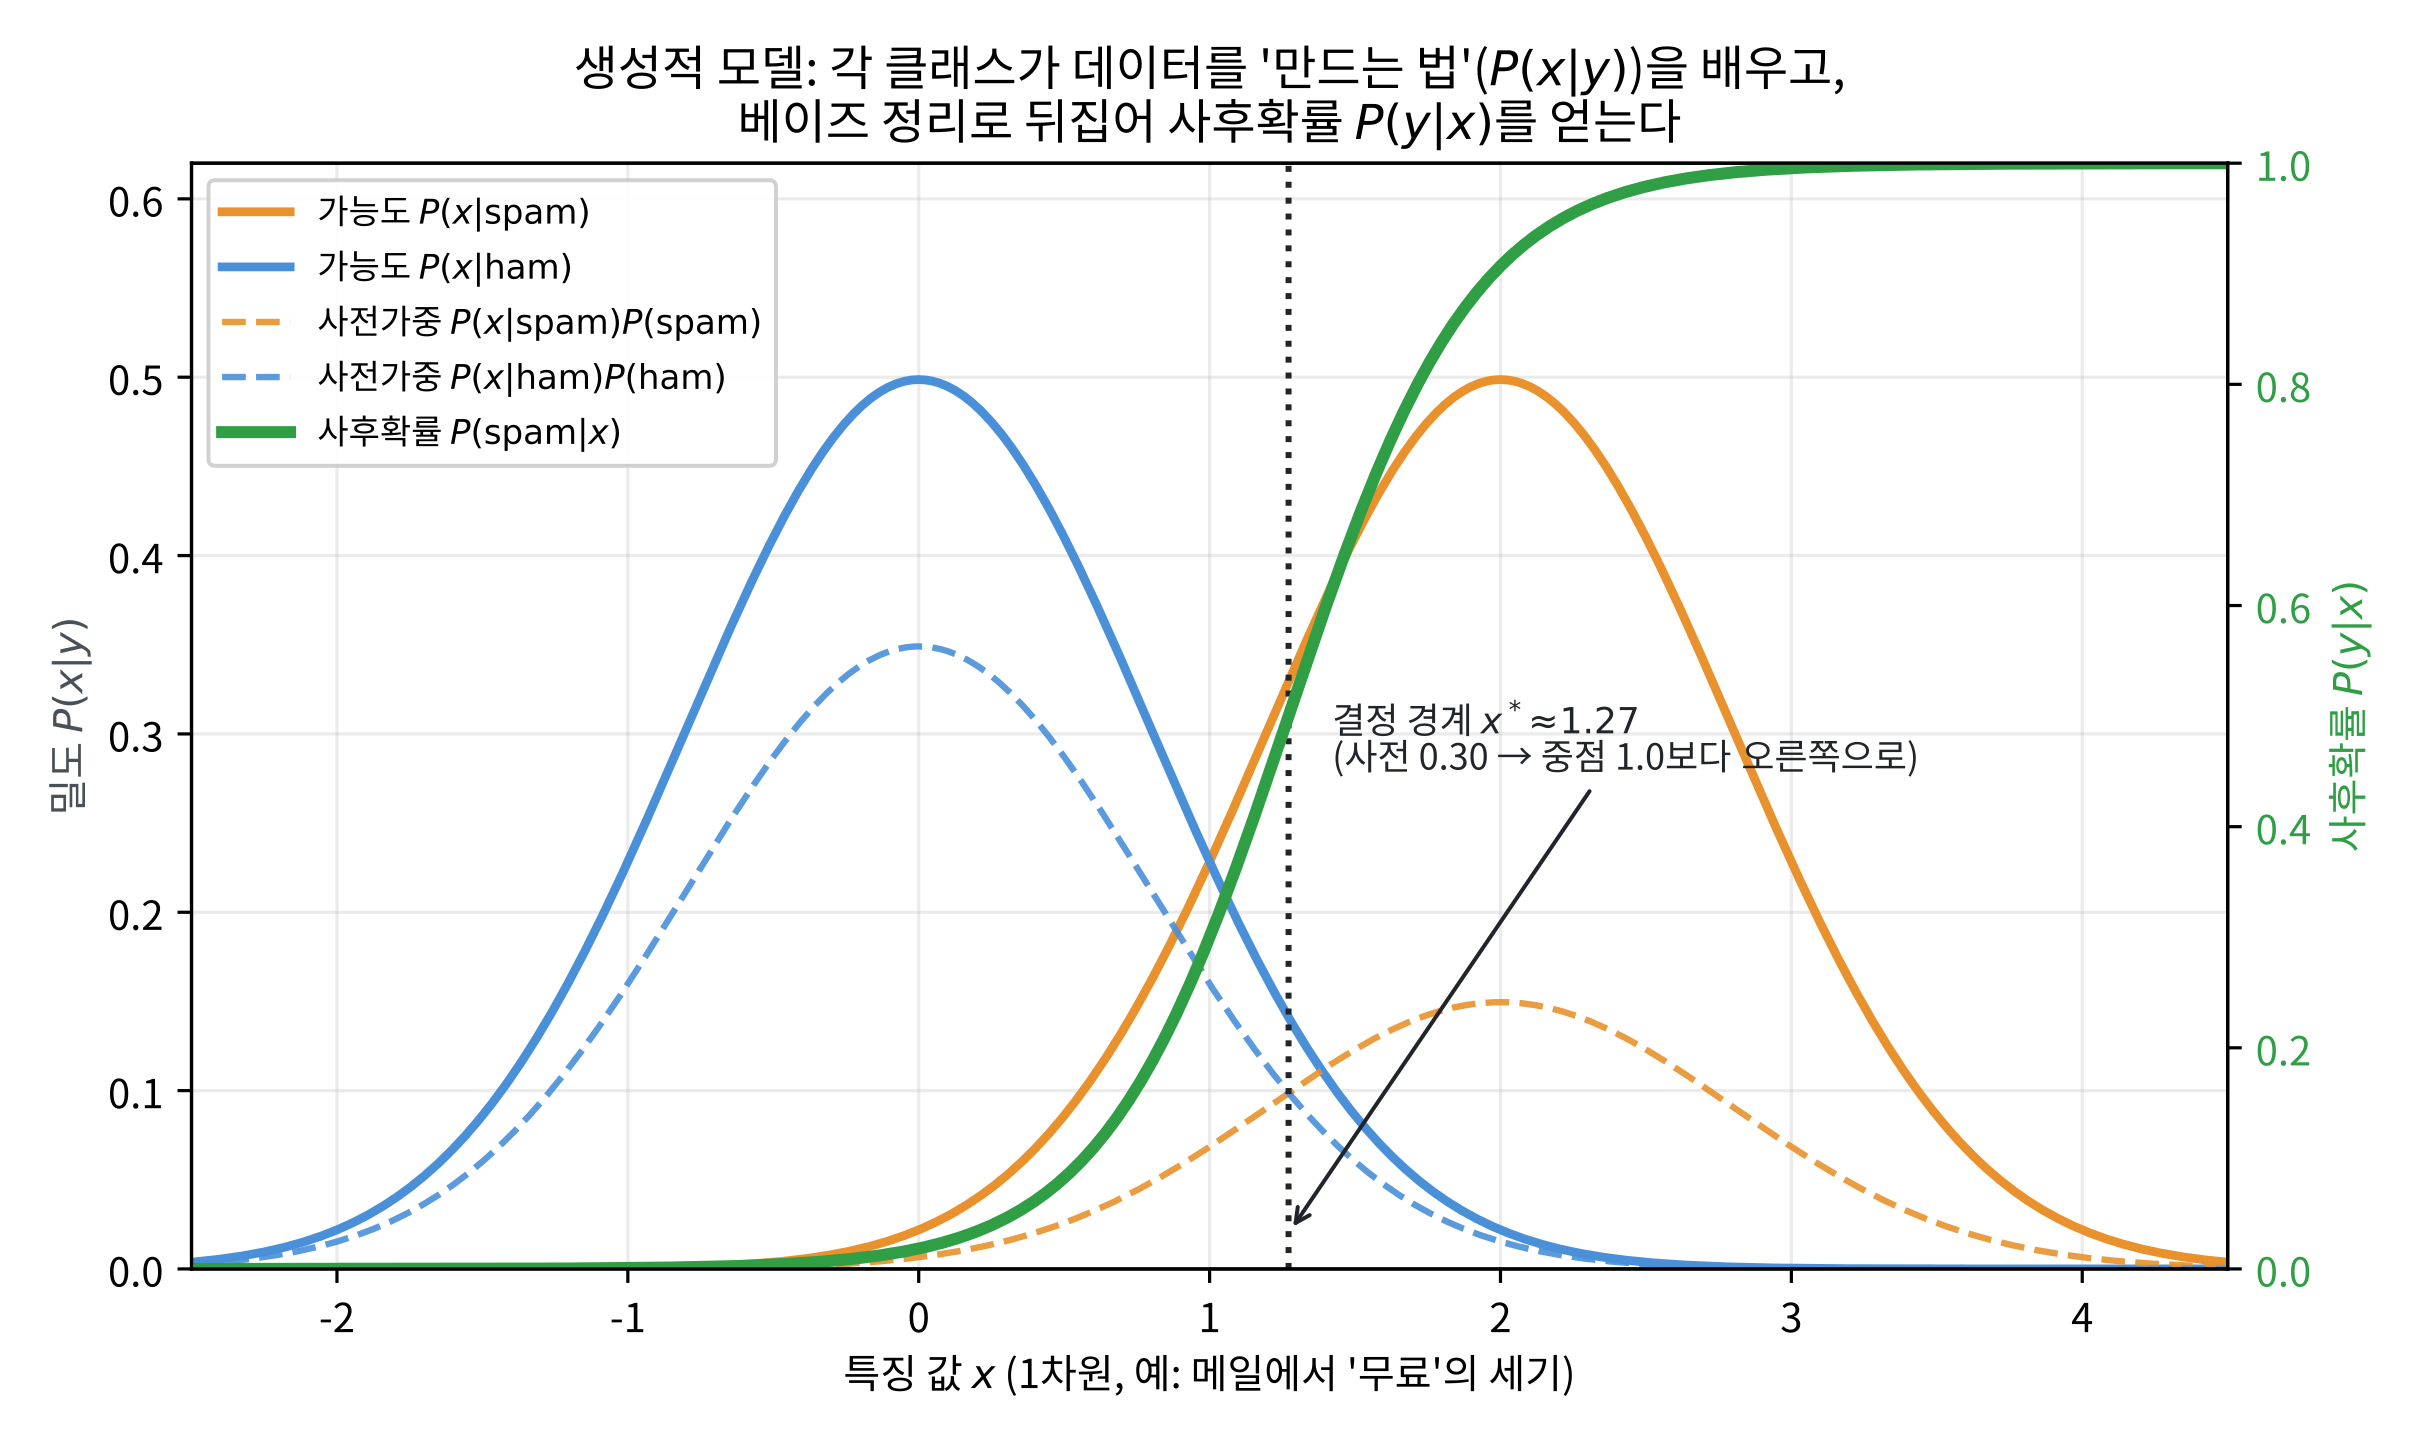
\includegraphics[width=\linewidth]{ch03_generative_vs_discriminative.png}
      \\[0.3em]{\footnotesize 가중 가능도 두 곡선의 교차점 $\approx$1.27이
      경계, 뒤집으면 사후확률 $P(\text{spam}|x)$.}
    \end{column}
  \end{columns}
\end{frame}

\begin{frame}{왜 베이즈 ``정리''가 필요한가}
  이 절의 모든 것이 이 한 줄에서 시작된다:
  \[ P(y|x) = \frac{P(x|y)P(y)}{P(x)} \]
  \vskip0.4em
  조건부확률의 정의 $P(x|y) = \frac{P(x,y)}{P(y)}$ 에서
  $P(x,y) = P(x|y)P(y)$ 로 고쳐 쓰고, 같은 $P(x,y)$ 를 반대 방향에서
  다시 나누면:
  \[ P(y|x) = \frac{P(x,y)}{P(x)} = \frac{P(x|y)P(y)}{P(x)} \]
  \vskip0.3em
  \begin{block}{``정리''가 아니라 ``계산''}
    새로운 사실이 아니라, \textbf{같은 결합확률 $P(x,y)$ 를 앞뒤로 나누는
    두 방법을 이어준 등식}.
  \end{block}
\end{frame}

\begin{frame}{뒤집기 문제(inversion problem)}
  \kq{왜 이 한 줄이 머신러닝에서 이토록 중요한가?}
  \vskip0.6em
  \begin{columns}[T]
    \begin{column}{0.5\textwidth}
      \kb{학습 가능 방향: $P(x|y)$}\\
      스팸 메일 뭉치를 꺼내 \textbf{단어 빈도를 세면} 되는 쪽 ---
      `무료'가 스팸에 등장할 확률.
    \end{column}
    \begin{column}{0.5\textwidth}
      \kb{필요 방향: $P(y|x)$}\\
      실제 작동할 때 필요한 쪽 --- `'무료'가 든 메일이 스팸일 확률''.
    \end{column}
  \end{columns}
  \vskip0.6em
  \begin{itemize}
    \item 두 방향이 \textbf{반대}인 문제를 \kb{뒤집기 문제}.
    \item 이 뒤집기를 가능하게 하는 다리는 \textbf{고유}.
    \item 3.2 GDA · 3.3 나이브베이즈 모두 이 다리를 건너는 모델.
    \item 3.2 끝: GDA의 사후확률이 \textbf{로지스틱회귀의 시그모이드와
      정확히 같은 형태}가 되는 것도 결국 ``베이즈 정리로 뒤집었다''에서
      나옴.
  \end{itemize}
\end{frame}

\begin{frame}{이름의 유래: Bayes(1701--1761)}
  \begin{itemize}
    \item \kb{리처드 베이즈}의 미발표 논문(사후에 1763년 발표)에서 나온
      아이디어.
    \item \kb{피에르-시몽 라플라스}가 체계화.
    \item 19$\sim$20세기에 \kb{``베이즈주의''}라는 확률 철학의 이름으로
      자리 잡음.
    \item 핵심 방식: \textbf{증거가 쌓일 때마다 확신을 갱신}.
    \item 실전에서 결정적 위력을 보인 사례(튜링의 에니그마 해독)는 이
      절 뒤에 다룸.
  \end{itemize}
\end{frame}

\begin{frame}{세 단어 + 증거: 하나의 이야기}
  \small
  \begin{tabular}{@{}ll@{}}
    \toprule
    용어 & 뜻(스팸 예) \\
    \midrule
    $P(y)$ \kb{사전확률} & 증거를 보기 \textbf{전에} 아는 비율 --- 스팸 30\%면 0.3 \\
    $P(x|y)$ \kb{가능도} & 클래스 주어졌을 때 증거가 나올 확률 --- `무료': 스팸 0.6, 정상 0.05 \\
    $P(y|x)$ \kb{사후확률} & 증거를 \textbf{보았을 때} 갱신된 확률 --- 분류에 쓰는 값 \\
    $P(x)$ \kb{증거(분할합)} & 어떤 클래스든 `무료'가 나올 전체 확률 --- \textbf{분류에선 약수로 사라짐} \\
    \bottomrule
  \end{tabular}
  \vskip1em
  \begin{block}{공통 어휘}
    이 네 단어는 Ch.\,15 EM/GMM, VAE(ELBO = Expected Lower Bound,
    ``사후확률의 기대 하한'')까지 이어지는 \textbf{공통 어휘} ---
    식을 볼 때마다 ``어디가 사전/가능도/사후인가''를 자동 짚을 것.
  \end{block}
\end{frame}

\begin{frame}{손으로 한 번: 스팸 확률 직접 계산}
  전체 메일의 30\%가 스팸($P(\text{spam})=0.3$), `무료'는 스팸 60\% ·
  정상 5\%로 등장.
  `무료'가 든 메일의 스팸 확률:
  \[ P(\text{spam}|\text{무료}) =
     \frac{0.6\times0.3}{0.6\times0.3 + 0.05\times0.7}
     = \frac{0.18}{0.18+0.035}
     = \frac{0.18}{0.215} \approx 0.837 \]
  \vskip0.4em
  \begin{block}{하나의 단어로}
    사전확률 \textbf{30\%} $\to$ 사후확률 \textbf{$\approx$83.7\%}로
    큰 도약. 이것이 나이브베이즈 필터의 본질. 3.3절에서는 이 계산을
    \textbf{모든 단어}에 대해(정확히는 로그를 \textbf{더해서}) 수행.
  \end{block}
\end{frame}

\begin{frame}{확률 없이: 사람(메일)을 세는 방식}
  1000통의 메일(스팸 300 · 정상 700)을 세어 보자:
  \small
  \begin{tabular}{@{}lcc@{}}
    \toprule
     & 스팸 (300통) & 정상 (700통) \\
    \midrule
    `무료' \textbf{들어감} & $300\times0.6=$ \textbf{180} & $700\times0.05=$ \textbf{35} \\
    `무료' 없음 & 120 & 665 \\
    \bottomrule
  \end{tabular}
  \vskip0.8em
  \begin{itemize}
    \item `무료'가 든 메일이라는 \textbf{조건}으로 세상을 좁히면
      총 215통(180+35), 그중 스팸 180통.
    \item $P(\text{spam}|\text{무료}) = 180/215 \approx 0.837$
      --- \textbf{빈도를 센 것만으로} 같은 답.
    \item \kb{확률 트리}: \textbf{세로 합(215)이 조건부 세계의 전체
      크기}, 그 안에서 원하는 칸(180)의 비율이 곧 사후확률.
    \item 의학과 보험, 사기 탐지 등 모든 베이즈 문제의
      \textbf{검증 도구}.
  \end{itemize}
\end{frame}

\begin{frame}{확률 트리로 보기}
  \begin{columns}[T]
    \begin{column}{0.55\textwidth}
      같은 계산을 나무 그림으로:
      \begin{itemize}
        \item ``조건에 맞는 열''(스팸 180 + 정상 35 = 215통)을
          \textbf{세로 합}해서 전체로 씀.
        \item 그 안에서 원하는 칸(스팸 180)의 비율을 읽으면
          사후확률.
        \item 기저율 오류의 의료 예에서도 같은
          트리/카운팅으로 검증.
      \end{itemize}
    \end{column}
    \begin{column}{0.43\textwidth}
      \centering
      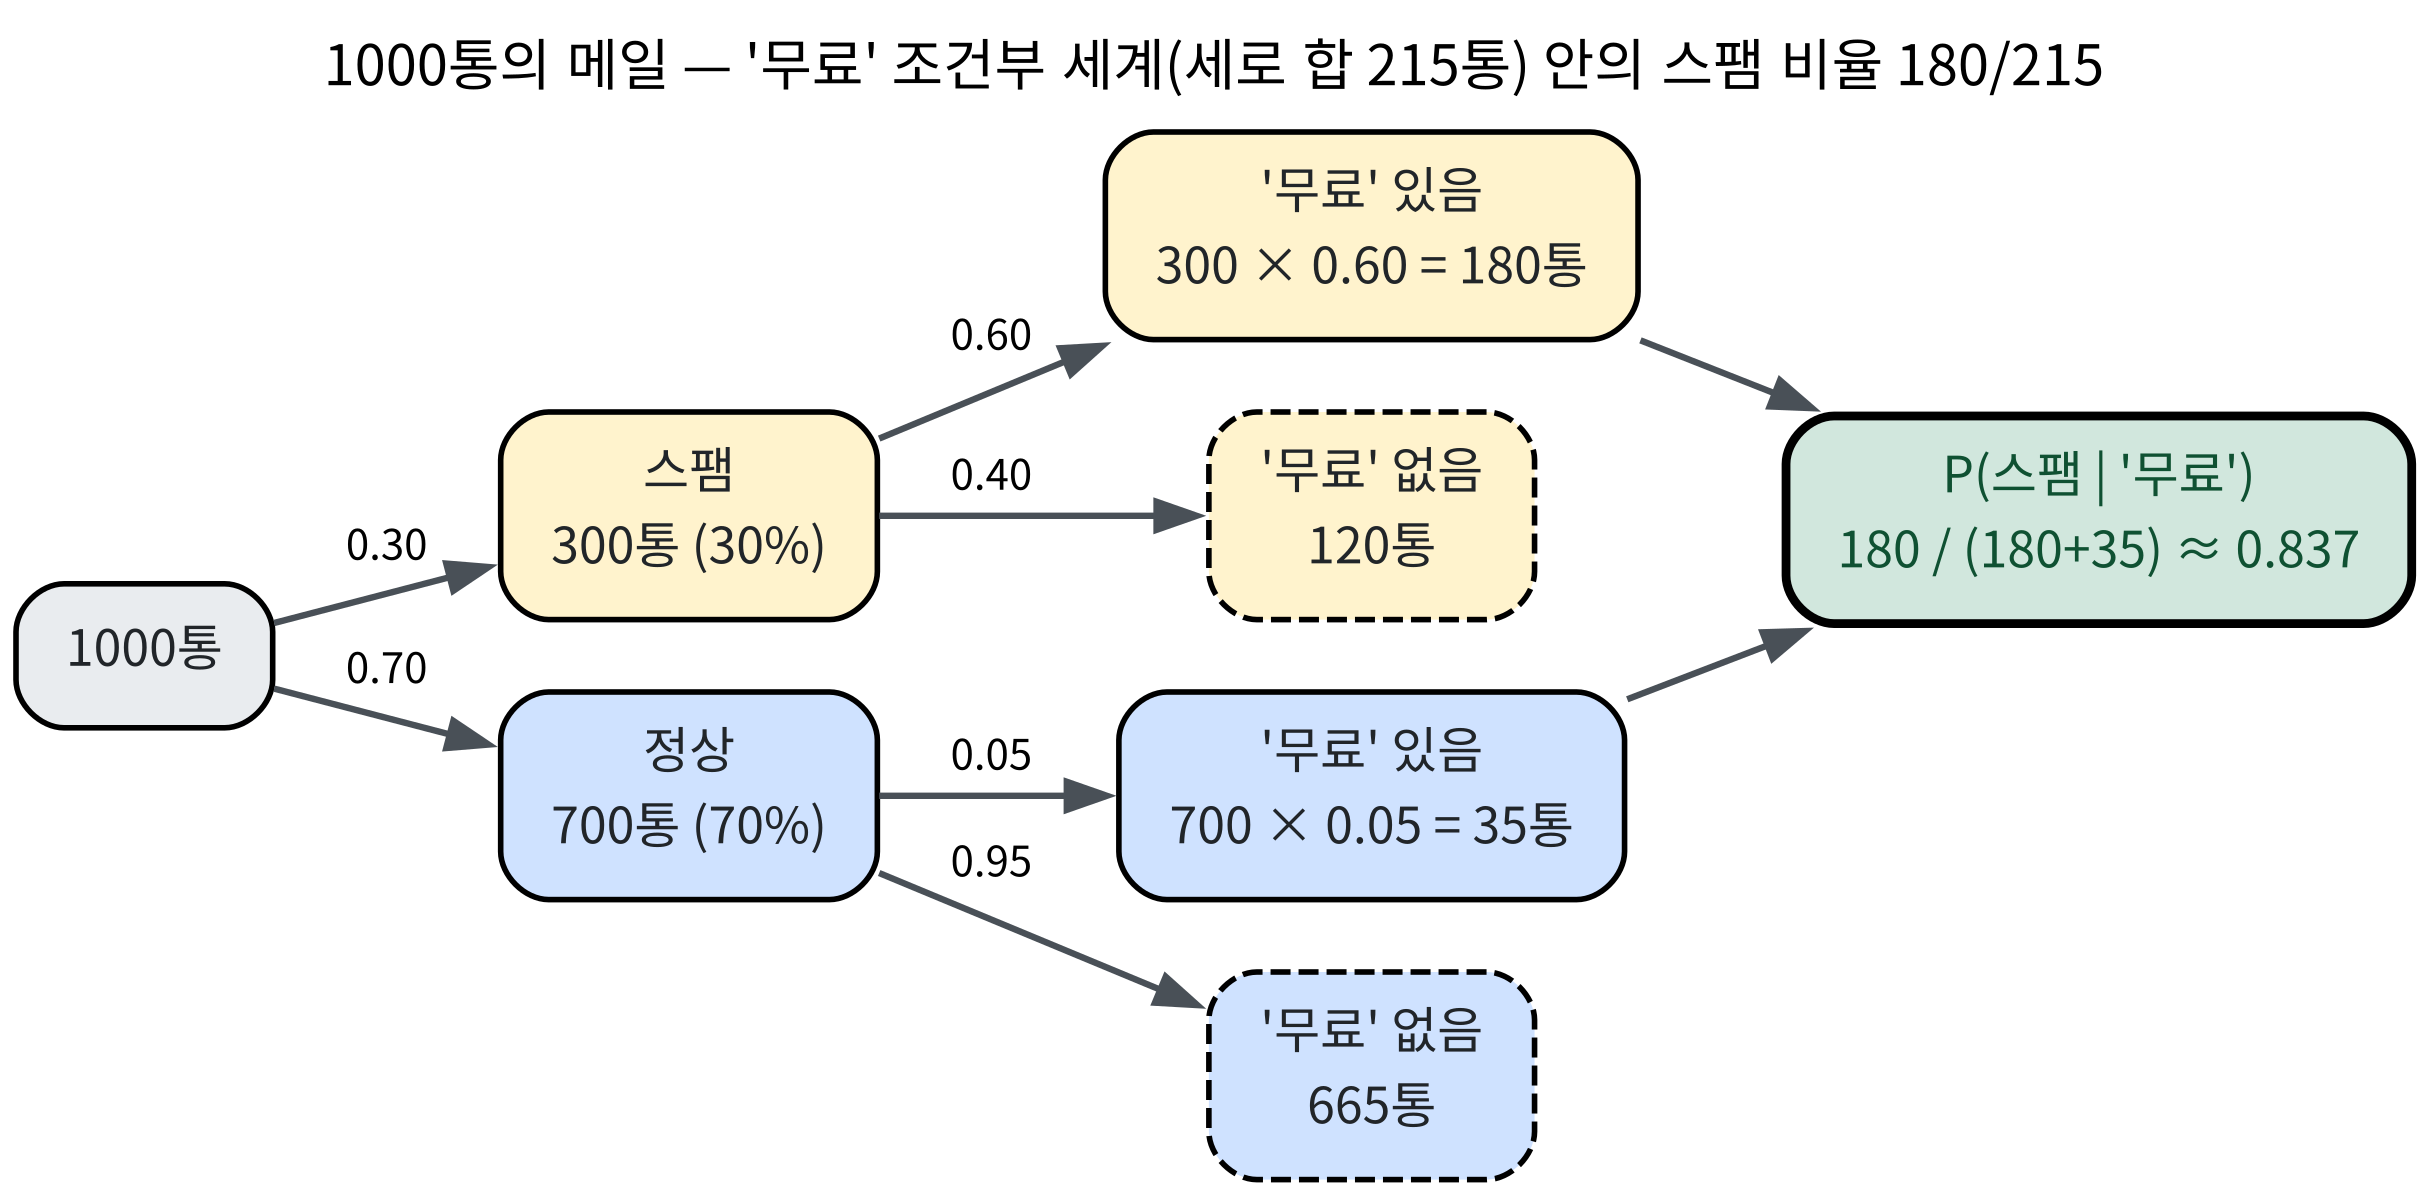
\includegraphics[width=\linewidth]{ch03_bayes_prob_tree.png}
      \\[0.3em]{\footnotesize `무료'가 든 215통의 조건부 세계 안에서
      스팸 비율 180/215 = 사후확률.}
    \end{column}
  \end{columns}
\end{frame}

\begin{frame}[fragile]{실습: 여러 증거를 곱해서 갱신}
  `무료'뿐 아니라 `당첨'도 등장했다면? 3.3절의 \kb{독립 가정}을
  미리 쓰면, 가능도를 \textbf{곱하기}만 하면 된다:
  \begin{lstlisting}
def bayes_update(prior_spam, likelihoods_spam, likelihoods_ham):
    """likelihoods_*: 관찰된 각 단어의 P(단어|클래스) 리스트"""
    p_spam = prior_spam
    for l_spam in likelihoods_spam:
        p_spam *= l_spam
    p_ham = 1 - prior_spam
    for l_ham in likelihoods_ham:
        p_ham *= l_ham
    return p_spam / (p_spam + p_ham)

# "무료"(0.6 vs 0.05)와 "당첨"(0.4 vs 0.02)이 함께 등장
result = bayes_update(0.3, [0.6, 0.4], [0.05, 0.02])
print(round(result, 4))  # 0.9904
  \end{lstlisting}
  \vskip0.2em
  {\footnotesize 증거가 하나 더해질수록 사후확률이 ``거의 확실히
  스팸''으로 쏠림 --- \textbf{순차적 추론}의 자연스러운 틀.}
\end{frame}

\begin{frame}{오즈(odds)로 다시 쓰기}
  베이즈 정리 양변을 $P(y)$ 로 나누면:
  \[ \frac{P(y|x)}{1-P(y|x)}
     = \frac{P(y)}{1-P(y)}\cdot\frac{P(x|y)}{P(x|1-y)} \]
  \vskip0.3em
  \begin{block}{사후오즈 = 사전오즈 $\times$ 가능도비}
    ``가능도를 곱한다''는 말은 정확히 이 한 줄
    (가능도비 = likelihood ratio, $P(x|y)/P(x|1-y)$).
  \end{block}
  \vskip0.3em
  \vskip0.4em
  \small
  스팸 예: 사전오즈 $0.3/0.7\approx0.43$에서 차례로 갱신:
  \begin{tabular}{@{}ll@{}}
    \toprule
    단계 & 오즈 $\to$ 확률 \\
    \midrule
    사전 & $\approx 0.43$ $\to$ 0.30 \\
    + `무료' $\times 12$ & $\approx 5.1$ $\to$ 0.837 \\
    + `당첨' $\times 20$ & $\approx 103$ $\to$ 0.990 \\
    \bottomrule
  \end{tabular}
\end{frame}

\begin{frame}{증거의 ``곱의 연쇄''}
  \begin{columns}[T]
    \begin{column}{0.55\textwidth}
      \begin{itemize}
        \item 증거가 하나씩 들어올 때마다 \textbf{오즈가 가능도비만큼만
          곱}해지며 갱신.
        \item 이 ``곱의 연쇄''가
        \begin{itemize}
          \item 3.3절: 나이브베이즈가 \textbf{로그를 더하는} 이유
          \item Ch.\,2: 로지스틱회귀가 \textbf{시그모이드를 쓰는} 이유
        \end{itemize}
        를 \textbf{같은 자리에서} 설명.
      \end{itemize}
    \end{column}
    \begin{column}{0.43\textwidth}
      \centering
      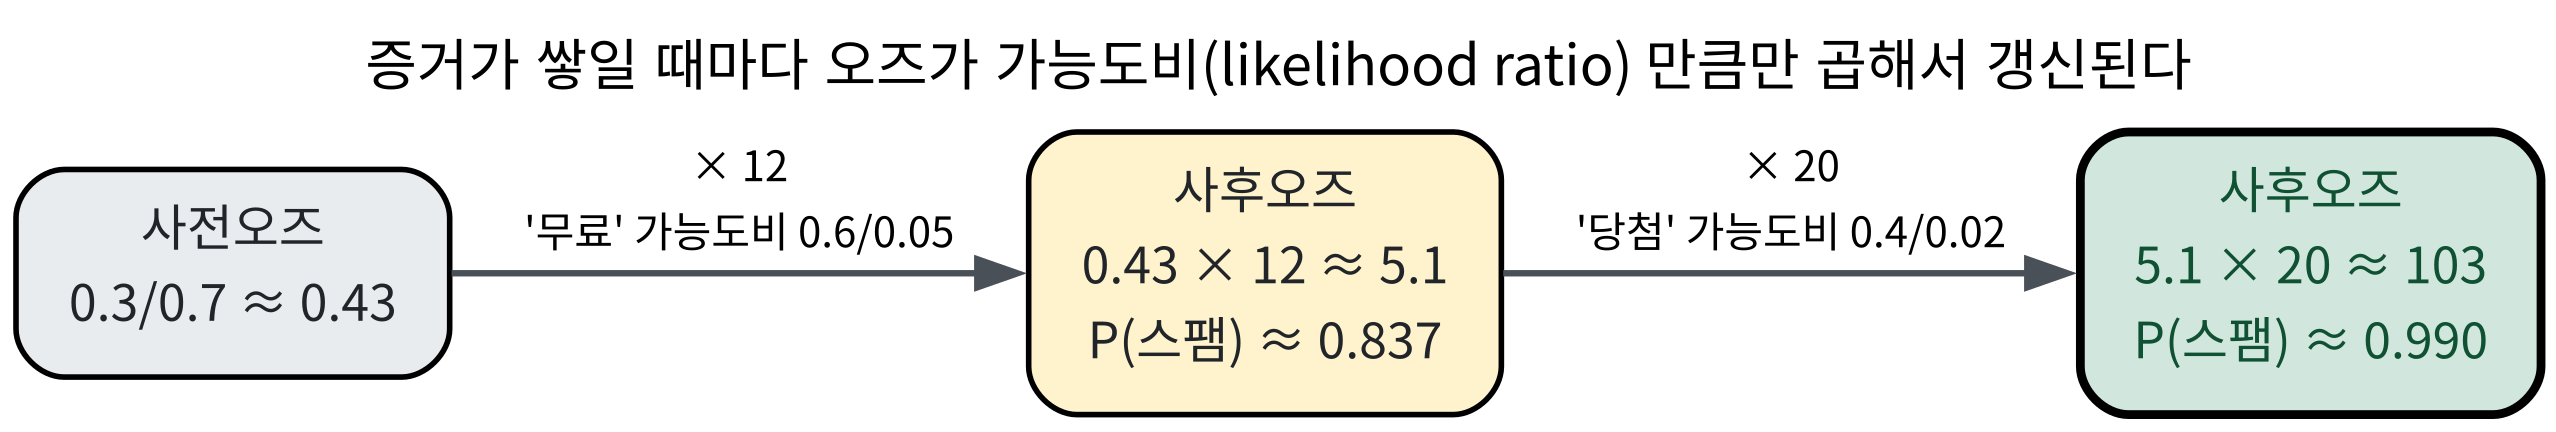
\includegraphics[width=\linewidth]{ch03_logodds_chain.png}
      \\[0.3em]{\footnotesize 사전오즈 0.43에 가능도비 12, 20을
      차례로 곱해 $\approx$103 ($\approx$0.990)까지.}
    \end{column}
  \end{columns}
\end{frame}

\begin{frame}{자주 하는 실수: 기저율 오류}
  \kq{가장 흔한 실수: 가능도 $P(x|y)$만 보고 사전확률 $P(y)$ 를 빼먹기.}
  \vskip0.5em
  의료 검진 예 --- 유병률 0.1\%, 검사 정확도 99\%:
  \[ P(\text{병}|\text{양성}) =
     \frac{0.99\times0.001}{0.99\times0.001 + 0.01\times0.999}
     = \frac{0.00099}{0.01098} \approx \textbf{0.090} \]
  \vskip0.3em
  \begin{itemize}
    \item 양성 나와도 실제로 병에 걸렸을 확률은 \textbf{$\approx$9\%}뿐.
    \item 1000명 검사: 병든 1명 중 진짜 양성 $\approx$1명, 건강한 999명 중
      가짜 양성 $\approx$10명.
    \item \textbf{가짜 양성 10 : 진짜 양성 1} 비율이 사후확률을 9\%로
      붙잡아 놓음.
    \item \kb{기저율 오류}(base rate fallacy) = 위양성의 역설:
      가능도가 아무리 높아도 사전확률이 낮으면 사후확률은 훨씬 낮음.
    \item 생성적 모델 실전에선 \textbf{사전확률 = 학습 데이터의 클래스
      비율}로 정확히 추정하는 게 중요.
  \end{itemize}
\end{frame}

\begin{frame}{기저율 오류를 1000명 세기로}
  \small
  \begin{tabular}{@{}lcc@{}}
    \toprule
     & 병 걸림 (1명) & 건강 (999명) \\
    \midrule
    검사 \textbf{양성} & $1\times0.99=$ \textbf{0.99} & $999\times0.01=$ \textbf{9.99} \\
    검사 음성 & 0.01 & 989.01 \\
    \bottomrule
  \end{tabular}
  \vskip0.8em
  \begin{itemize}
    \item ``양성''으로 좁히면 총 10.98명, 그중 병든 0.99명 ---
      $0.99/10.98 \approx 0.090$, 확률 계산과 \textbf{완전히 같은 답}.
    \item ``검사 정확도가 99\%인데 왜 사후확률이 9\%인가'' ---
      \textbf{가짜 양성과 진짜 양성의 비율}로 설명.
    \item 스팸 예의 확률 트리와 \textbf{동일한 구조}로 검증.
  \end{itemize}
\end{frame}

\begin{frame}{유명한 사례: 튜링과 에니그마}
  \begin{itemize}
    \item 2차대전, 영국 블레츨리 파크 --- 앨런 튜링과 동료들이 독일군
      \kb{에니그마} 암호를 깨기 위해, 각 암호 설정의 ``가능성''을
      \textbf{베이즈적으로 갱신}.
    \item 튜링이 확률 갱신량의 단위를 ``\kb{반(ban)}''이라고 불렀는데,
      이것은 정확히 \kb{로그 가능도비}(log-likelihood ratio)와 같은 개념.
    \item 새 암호문 조각(증거)이 들어올 때마다 각 설정의 사후확률을
      갱신 --- 가능한 설정을 사실상 무한대 $\to$ 실용적 범위까지 축소.
    \item 정답을 몰라도 ``증거가 쌓일수록 확신이 어떻게 바뀌는가''를
      수학적으로 다루는 방식 --- 스팸 필터의 단어 하나하나와
      \textbf{원리적으로 동일}.
  \end{itemize}
\end{frame}

\begin{frame}{자주 묻는 질문 (3.1)}
  \begin{columns}[T]
    \begin{column}{0.5\textwidth}
      \textbf{Q1. 생성 vs 판별, 뭐가 더 좋은가?}
      \begin{itemize}
        \item \textbf{데이터 적을 때}: 생성적(GDA, 나이브베이즈) ---
          ``클래스가 데이터를 어떻게 만드나''라는 \textbf{강한 가정}을
          깔고 들어가 적은 데이터로도 안정적.
        \item \textbf{데이터 많을 때}: 판별적(로지스틱회귀) ---
          가정 없이 직접 경계 학습 $\Rightarrow$ 가정 틀림 위험 없음.
        \item 3.2절에서 GDA와 로지스틱회귀가 \textbf{같은 형태의
          결정 경계}로 수렴함을 직접 확인.
        \item 더 깊이: Stanford CS229 노트.
      \end{itemize}
    \end{column}
    \begin{column}{0.5\textwidth}
      \textbf{Q2. $P(x)$ 를 왜 무시해도 되나?}
      \begin{itemize}
        \item 분류에서는 \textbf{고정된 $x$ 하나}를 놓고
          ``$y=0$ 이 맞을까, $y=1$ 이 맞을까''만 비교.
        \item $P(x)$ 는 어떤 클래스를 비교하든 \textbf{항상 같은 값}
          (분모가 같으면 분자만 비교해도 대소관계 유지).
        \item 그래서 \textbf{분자 $P(x|y)P(y)$ 만 최대화}하는 클래스를
          고르면 충분.
      \end{itemize}
    \end{column}
  \end{columns}
\end{frame}

% =================================================================
\section{3.2 가우시안 판별분석 (GDA)}

\begin{frame}{왜 가우시안인가: 가장 자연스러운 가정}
  3.1절: 생성적 분류기는 $P(x|y)$ 를 먼저 모델링하고 뒤집는다.
  이 `만드는 법'을 쓰려면 $x$ 에 대한 \textbf{구체적 분포}를 골라야 한다.
  \vskip0.5em
  \begin{itemize}
    \item $x$ 가 \textbf{이산}(단어 등장 여부)이면 --- 빈도 카운팅
      $\Rightarrow$ 3.3절 \kb{나이브베이즈}.
    \item $x$ 가 \textbf{연속}(키, 공부 시간, 픽셀)이면 ---
      \kb{가우시안 분포}(정규분포).
  \end{itemize}
  \vskip0.4em
  \textbf{이유 두 가지:}
  \begin{enumerate}
    \item 평균 $\mu$ 와 공분산 $\Sigma$ 두 파라미터만으로 ``중심 위치''+
      ``퍼짐'' 표현 --- \textbf{간결}.
    \item 현실의 연속 측정값은 수많은 작은 효과의 합 ---
      \kb{중심극한정리}로 가우시안에 가까워지는 경향.
  \end{enumerate}
  각 클래스를 가우시안으로 모델링하는 분류기 = \kb{GDA}.
\end{frame}

\begin{frame}{이진 GDA의 모델: 공유 공분산}
  \[ y \sim \mathrm{Bernoulli}(\phi), \hspace{2em}
     x\mid y{=}0 \sim \mathcal{N}(\mu_0,\Sigma), \hspace{2em}
     x\mid y{=}1 \sim \mathcal{N}(\mu_1,\Sigma) \]
  \vskip0.4em
  \begin{itemize}
    \item 두 클래스가 \textbf{같은 공분산 행렬 $\Sigma$ 를 공유}하되
      평균 $\mu_0,\mu_1$ 만 다름.
    \item 직관: 같은 ``모양''으로 퍼져 있고 \textbf{중심 위치만 다른}
      두 구름.
    \item 파라미터 $\phi,\mu_0,\mu_1,\Sigma$ 는 학습 데이터의
      \textbf{평균·공분산을 그대로 계산}해서 구함 (최대우도추정,
      MLE).
    \item \textbf{경사하강법 없이 닫힌 형태}로 바로 구해짐 ---
      로지스틱회귀와의 실전적 차이.
  \end{itemize}
\end{frame}

\begin{frame}{파라미터 추정: MLE가 왜 단순해지는가}
  \kb{최대우도추정}(MLE) --- 데이터를 ``가장 그럴듯하게'' 설명하는
  파라미터. 데이터 독립이면:
  \[ \ell = \sum_{i:\,y_i=0}\log P(x_i|y{=}0)
     + \sum_{i:\,y_i=1}\log P(x_i|y_i{=}1)
     + \sum_i\big[y_i\log\phi + (1-y_i)\log(1-\phi)\big] \]
  \vskip0.3em
  각 파라미터로 \textbf{편미분 $\to$ 0}을 풀면, 해가 놀랍도록 단순한
  \textbf{샘플 통계량}으로 나옴:
  \begin{itemize}
    \item $\hat\phi$ = 학습 데이터 중 $y{=}1$ 의 \textbf{비율}
      (사전확률 추정).
    \item $\hat\mu_0,\hat\mu_1$ = 클래스별 \kb{샘플 평균}.
    \item $\hat\Sigma$ = 두 클래스의 \textbf{클래스 평균 기준 편차를
      함께 모아}(pooling) 제곱평균:
    \[ \hat\Sigma = \frac{1}{N}\sum_{i=1}^{N}
       (x_i-\hat\mu_{y_i})(x_i-\hat\mu_{y_i})^\top \]
  \end{itemize}
\end{frame}

\begin{frame}{닫힌 형태의 의미: 대입하는 순간 끝}
  \begin{itemize}
    \item $\hat\mu_{y_i}$ = 샘플 $i$ 가 속한 \textbf{클래스의 평균}.
    \item 분모가 클래스별 $n_0,n_1$ 이 아니라 \textbf{전체 $N=n_0+n_1$}
      --- 바로 두 클래스의 편차를 \textbf{합쳐서} 평균내기.
    \item 1차원 예시의 ``편차 6개를 한꺼번에 나누던 것''과 같은 절차.
    \item 로지스틱회귀: 경사하강으로 $w,b$ 를 \textbf{반복 탐색}
      vs GDA: 수식에 \textbf{대입하는 순간 파라미터 끝}.
    \item Ch.\,2.2 정규방정식의 ``한 번에 풀기''와 같은 계열.
    \item {\footnotesize (세세한 차이: 통계학에선 $N{-}d{-}1$ 로 나누어
      편향을 없애는 버전도 있지만, 학습엔 위 MLE 버전이 표준,
      데이터가 크면 차이 없음.)}
  \end{itemize}
\end{frame}

\begin{frame}{손으로 한 번: 1차원 GDA로 결정 경계}
  공부 시간으로 시험 합격/불합격 예측 ---
  불합격 $[2,3,4]$, 합격 $[6,7,8]$ (크기 같아 $\phi=0.5$).
  \vskip0.4em
  \[ \mu_0 = \frac{2+3+4}{3} = 3, \hspace{2em} \mu_1 = \frac{6+7+8}{3} = 7 \]
  \vskip0.2em
  공유 분산 --- 두 그룹의 \textbf{클래스 평균 기준 편차 6개를 함께}
  제곱평균:
  \[ \sigma^2 = \frac{1+0+1+1+0+1}{6} = \frac{2}{3} \approx 0.667 \]
  \vskip0.3em
  \begin{block}{사전확률이 50:50이면}
    결정 경계(사후확률이 같아지는 지점) = 두 평균의 \textbf{정확한 중점}:
    \[ x^{*} = \frac{\mu_0+\mu_1}{2} = \frac{3+7}{2} = \textbf{5} \]
  \end{block}
\end{frame}

\begin{frame}{$x^{*}=5$ 를 밀도로 검증}
  \small
  \begin{tabular}{@{}cccc@{}}
    \toprule
    $x$ & $P(x|y{=}0)$ 에 비례 & $P(x|y{=}1)$ 에 비례 & 예측 \\
    \midrule
    4.5 & 0.0452 & 0.0022 & 0 (불합격) \\
    5.0 & 0.0122 & 0.0122 & 경계 (동점) \\
    5.5 & 0.0022 & 0.0452 & 1 (합격) \\
    \bottomrule
  \end{tabular}
  \vskip1em
  \begin{itemize}
    \item 정확히 $x{=}5$ 를 기준으로 \textbf{예측이 뒤집힘} ---
      손으로 구한 $x^{*}=5$ 와 정확히 일치.
    \item 실전 GDA는 다차원 $\to$ $\sigma^2$ 대신 공분산 \textbf{행렬}
      $\Sigma$ 를 쓰지만, ``두 평균의 중점 근처에서 경계가 생긴다''는
      직관은 \textbf{그대로 유지}.
  \end{itemize}
\end{frame}

\begin{frame}{결정 경계의 모양: 왜 항상 직선인가}
  \kb{로그 우도비}로 경계 규칙을 쓰면 ---
  $P(y{=}1|x) > P(y{=}0|x)$ 인가? $\Leftrightarrow$ $z(x) > 0$ 인가?:
  \[ z(x) = \log\frac{P(y{=}1|x)}{P(y{=}0|x)}
     = -\tfrac12(x-\mu_1)^\top\Sigma^{-1}(x-\mu_1)
       + \tfrac12(x-\mu_0)^\top\Sigma^{-1}(x-\mu_0)
       + \log\tfrac{\phi}{1-\phi} \]
  \vskip0.3em
  \begin{block}{핵심 한 줄}
    $(x{-}\mu)^\top\Sigma^{-1}(x{-}\mu)$ 를 전개하면
    $x^\top\Sigma^{-1}x$ 항이 \textbf{두 클래스 모두}에 등장하는데,
    $\Sigma$ 를 공유하므로 이 \textbf{이차항이 정확히 상쇄}.
    남는 것은 $x$ 에 대한 \textbf{일차식}뿐.
  \end{block}
\end{frame}

\begin{frame}{직선의 $w$ 와 $b$}
  \[ z(x) = w^\top x + b \]
  \[ w = \Sigma^{-1}(\mu_1 - \mu_0), \hspace{2em}
     b = -\tfrac12(\mu_1{-}\mu_0)^\top\Sigma^{-1}(\mu_1{+}\mu_0)
         + \log\tfrac{\phi}{1{-}\phi} \]
  \vskip0.4em
  결정 경계 $z(x)=0$ 은 \textbf{직선}($d$ 차원이면 초평면) ---
  ``\kb{선형} 판별''이라는 이름이 여기서 옴.
  \vskip0.4em
  \begin{itemize}
    \item $\Sigma_0 \ne \Sigma_1$ 이면(공유 안 하면) 이차항이 안 상쇄
      $\to$ \textbf{곡선}(쌍곡선) 경계 = \kb{QDA}
      (이차판별분석, 연습문제 2 참고).
  \end{itemize}
\end{frame}

\begin{frame}{$w$ 의 방향: 마할라노비스 보정}
  \begin{itemize}
    \item $w$ 의 방향은 \kb{마할라노비스 거리}로 두 평균을 잇는 방향
      --- $\Sigma^{-1}$ 이 데이터의 \textbf{퍼진 모양에 맞게 방향을
      보정}하기 때문.
    \item 데이터가 $x_1$ 축 방향으로 \textbf{넓게 퍼져} 있으면,
      그 방향의 차이는 구별력에 기여가 적으므로 $\Sigma^{-1}$ 이
      그 방향의 기여를 \textbf{줄여}줌.
    \item 반대로 좁게 모인 방향은 \textbf{증폭}.
    \item 특별한 경우 $\Sigma = \sigma^2 I$ (원형, 방향 없음):
      $w$ 는 그냥 $\mu_1{-}\mu_0$ 에 \textbf{비례} ---
      ``두 평균을 잇는 수직선에 경계''라는 초보 직관이 그대로 성립.
  \end{itemize}
\end{frame}

\begin{frame}{$\phi$ 는 위치만, 기울기는 그대로}
  \begin{itemize}
    \item \kb{사전확률 $\phi$ 는 방향이 아니라 위치($b$)만 움직인다.}
    \item $\phi$ 는 $\log\frac{\phi}{1-\phi}$ 항에만 등장 ---
      클래스 비율이 무엇이든 \textbf{직선의 기울기는 그대로},
      \textbf{밀리는 정도}만 바뀜.
    \item 다음 ``가정이 깨질 때'' 절에서 이 효과를 \textbf{숫자로}
      확인.
  \end{itemize}
  \vskip0.6em
  {\footnotesize (전개 과정의 전체 유도 = 이번 장 연습문제 2번.
  ``정확성 확인''에서 $\Sigma_0\ne\Sigma_1$ 이면 이차항 미상쇄
  $\to$ 곡선 = QDA.)}
\end{frame}

\begin{frame}{로지스틱회귀와 만나는 지점}
  \begin{block}{놀라운 사실 (Ng \& Jordan, 2001)}
    이렇게 구한 $P(y{=}1|x)$ 를 베이즈 정리로 전개하면, 정확히
    Ch.\,2 로지스틱회귀의 \textbf{같은 시그모이드 형태}
    \[ P(y{=}1|x) = \sigma(w^\top x + b) \]
    가 나온다.
  \end{block}
  \vskip0.5em
  \begin{itemize}
    \item GDA = ``로지스틱회귀와 같은 결정 경계(직선)에 도달하는
      \textbf{또 다른 길}''.
    \item \textbf{트레이드오프}: 데이터가 실제로 가우시안에 가까우면
      GDA가 적은 데이터로도 잘 맞고, 가정이 틀렸으면 판별적
      (로지스틱회귀)이 더 안정적.
    \item ``모델을 데이터에 맞출 것인가, 데이터가 모델을 따르는가'' ---
      생성적 vs 판별적의 근본적 갈림.
    \item 아래 ``실현'' 절에서 수치로 확인: 2차원 가우시안 데이터에서
      GDA의 닫힌 형태 $w,b$ 와 경사하강 로지스틱 $w,b$ 는
      \textbf{거의 같은 방향}.
  \end{itemize}
\end{frame}

\begin{frame}{유명한 사례: 피셔의 1936년 선형 판별}
  GDA는 기계학습 시대의 모델이 아니다 ---
  \kb{피셔}(Ronald Fisher, 1936)의 ``분류 문제에서 다중 측정의 이용''
  (아이리스 꽃의 종을 꽃술·꽃잎 길이/너비로 분류).
  \vskip0.4em
  \begin{itemize}
    \item 아이디어: 꽃을 단일 숫자 $z=w^\top x$ 로 ``꾀서'',
      \textbf{종 간 중심 거리 $\div$ 종 내부 퍼짐}을 \textbf{최대화}하는
      $w$ 를 찾는다:
    \[ \max\;\frac{w^\top S_B w}{w^\top S_W w} \;\;(\text{레이리 코시언트}) \]
    \item 최적 방향: $w \propto S_W^{-1}(\mu_1{-}\mu_0)$
      --- \textbf{공유 공분산 GDA의 $w$ 와 정확히 같은 방향}.
    \item ``가우시안 모델 + 베이즈 뒤집기'' 경로와 ``분류 성능을
      기하학적으로 최적화'' 경로가 \textbf{같은 직선}을 내놓음
      --- 가우시안 가정이 ``잘못된 모양''이 아님을 보여주는 증거.
    \item 이 모델 = 오늘날 \kb{피셔 선형 판별(LDA)}. 이진 분류 +
      공유 공분산이면 ``피셔 LDA''와 ``GDA''는 \textbf{동일한 모델}.
  \end{itemize}
\end{frame}

\begin{frame}[fragile]{실현: numpy로 GDA 구현}
  \begin{lstlisting}
import numpy as np

def fit_gda(X, y):
    """GDA 파라미터 (phi, mu0, mu1, Sigma)의 최대우도추정."""
    phi = y.mean()                                  # P(y=1) 추정
    mu0, mu1 = X[y == 0].mean(axis=0), X[y == 1].mean(axis=0)
    d0, d1 = X[y == 0] - mu0, X[y == 1] - mu1
    Sigma = (d0.T @ d0 + d1.T @ d1) / len(X)        # 두 클래스 편차 pooling
    return phi, mu0, mu1, Sigma

def gda_scores(X, phi, mu0, mu1, Sigma):
    """log P(y=1|x)/P(y=0|x) = w^Tx + b  (결정 경계는 직선!)"""
    Sigma_inv = np.linalg.inv(Sigma)
    w = Sigma_inv @ (mu1 - mu0)
    b = -0.5 * (mu1 - mu0) @ Sigma_inv @ (mu1 + mu0) + np.log(phi / (1 - phi))
    return X @ w + b, w, b
  \end{lstlisting}
  \vskip0.2em
  {\footnotesize $fit\_gda$ = MLE(닫힌 형태), $gda\_scores$ = 로그
  우도비 $z(x)=w^\top x+b$.}
\end{frame}

\begin{frame}{2차원 GDA 시각화}
  \begin{columns}[T]
    \begin{column}{0.55\textwidth}
      \begin{itemize}
        \item 2차원 가우시안 300+300개 샘플로 검증:
          참 평균 $[1,2]$, $[4,5]$, 참 공분산
          $\begin{bmatrix}1.5&0.8\\0.8&1.2\end{bmatrix}$.
        \item 추정 $\hat\mu_0,\hat\mu_1$ 이 참 평균에
          \textbf{접근} (300개 표본이라 노이즈 $\pm0.1$ 정도).
        \item 결정 경계 = $w_0 x_1 + w_1 x_2 + b = 0$ 인 \textbf{직선}.
        \item 기울기는 공분산의 ``퍼진 방향''에 맞춰 보정된 $w$ 가
          결정.
      \end{itemize}
    \end{column}
    \begin{column}{0.43\textwidth}
      \centering
      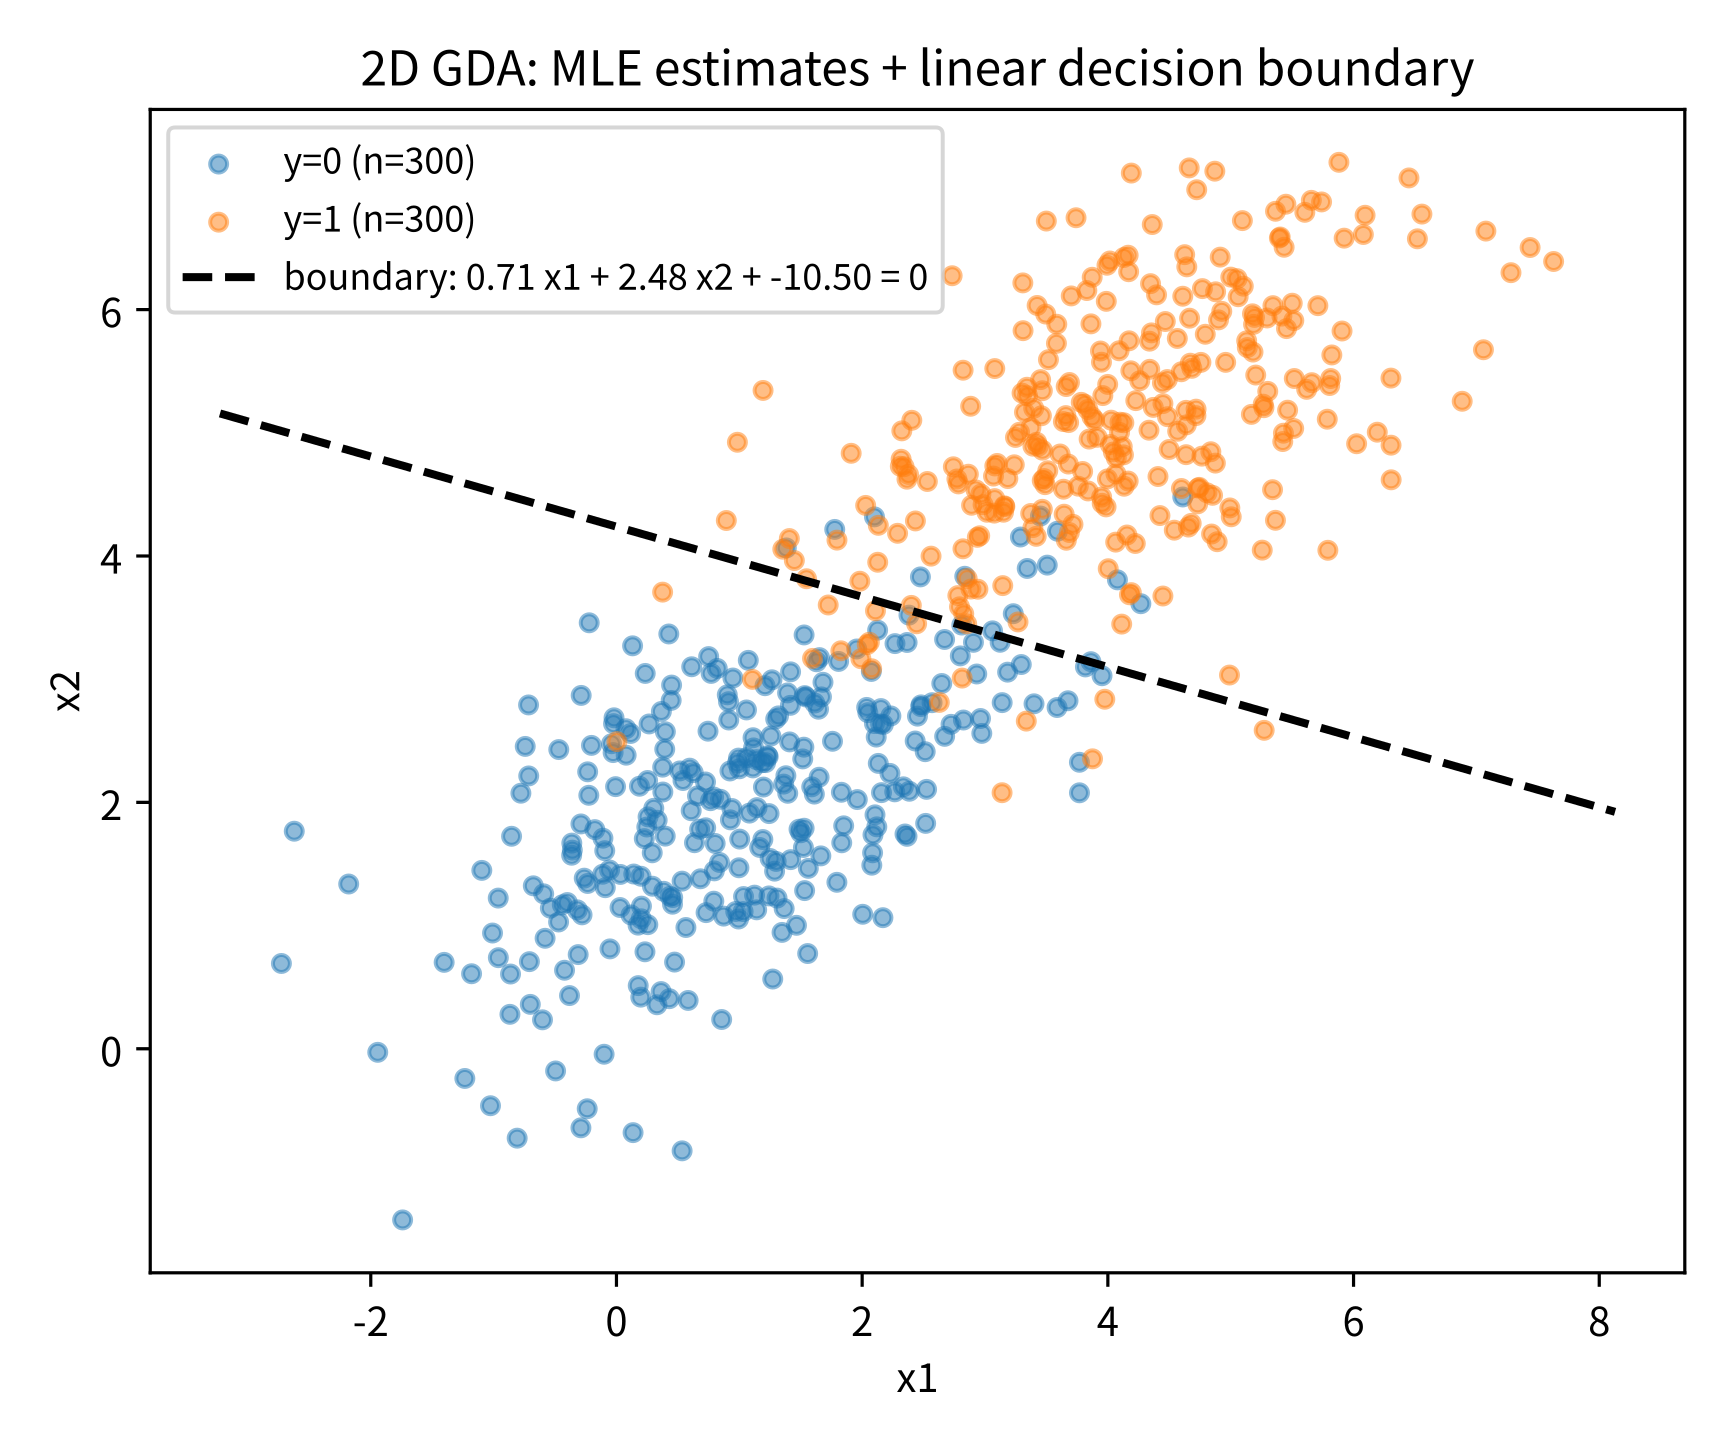
\includegraphics[width=\linewidth]{ch03_2_gda_boundary.png}
      \\[0.3em]{\footnotesize MLE로 추정한 두 클래스 가우시안과
      결정 경계 직선(검은 점선).}
    \end{column}
  \end{columns}
\end{frame}

\begin{frame}[fragile]{실습: sklearn LDA로 GDA 확인}
  scikit-learn의 \kb{LinearDiscriminantAnalysis}(LDA)가 정확히
  ``공분산을 공유하는'' GDA에 해당 --- 손 계산 예로 확인:
  \begin{lstlisting}
import numpy as np
from sklearn.discriminant_analysis import LinearDiscriminantAnalysis

X = np.array([[2.0], [3.0], [4.0], [6.0], [7.0], [8.0]])
y = np.array([0, 0, 0, 1, 1, 1])

lda = LinearDiscriminantAnalysis()
lda.fit(X, y)
print(lda.predict([[4.5], [5.0], [5.5]]))   # [0 0 1] (5.0 근처가 경계)
print(lda.means_)                            # [[3.] [7.]]
  \end{lstlisting}
  \vskip0.2em
  {\footnotesize $lda.means_ = [3,7]$ --- 손으로 구한 $\mu_0{=}3,
  \mu_1{=}7$ 과 정확히 일치. \textbf{실제 predict 출력은 $[0,0,1]$} ---
  $x{=}5.0$ 은 경계 위 동점이므로 sklearn은 ``동점이면 클래스 0'' 규칙
  적용. numpy GDA와 sklearn LDA를 2차원에서 함께 돌리면 $w$ 방향이
  동일하고 예측도 거의 모든 점에서 일치(확률값만 스케일 상수 차이).}
\end{frame}

\begin{frame}{가정이 깨질 때: 불균형 사전확률}
  ``$\phi$ 는 위치만 미는 게 얼마나 큰가''를 숫자로 ---
  앞의 예($\mu_0{=}3,\mu_1{=}7,\sigma^2{=}2/3$)에 ``매우 어려운 시험''
  ($\phi_0{=}0.8$ 불합격, $\phi_1{=}0.2$ 합격)을 대입:
  \[ z(x) = 6x - 30 + \log\tfrac{0.2}{0.8} \]
  \vskip0.2em
  ($6x{-}30$ = $(x{-}3)^2$ 과 $(x{-}7)^2$ 의 이차항 상쇄 결과,
  마지막 항 = 사전확률의 로그비). 경계 $z(x)=0$:
  \[ x^{*} = \frac{30 + \log(0.8/0.2)}{6}
     = \frac{30 + 1.386}{6} \approx \textbf{5.23} \]
  \vskip0.3em
  50:50일 때 경계 $x^{*}=5$ 였는데, 불합격 80\%로 \textbf{경계 5.23으로
  밀림} --- \textbf{소수 클래스(합격) 쪽으로}.
\end{frame}

\begin{frame}{경계의 물리적 이동 = 기저율 오류}
  \begin{itemize}
    \item 분류기가 소수 클래스에 대해 \textbf{보수적}이 됨.
    \item 3.1절 \kb{기저율 오류}와 정확히 같은 이야기:
      ``증거(가능도)가 아무리 강해도 사전확률이 낮으면 사후확률은
      기대만큼 안 올라간다''가 \textbf{결정 경계가 물리적으로
      이동하는} 형태로 나타남.
    \item 실전 클래스 비율 9:1이면 GDA는 ``소수 클래스로 예측하기
      전에 \textbf{더 확실한 증거}를 요구''하며 자동으로 경계를 옮겨줌.
    \item 실습 노트북에서는 2차원으로 시각화 --- 기울이는 같은 직선이
      $\phi$ 값에 맞게 \textbf{병렬 이동}.
  \end{itemize}
\end{frame}

\begin{frame}{자주 하는 실수: 공유 공분산 가정}
  GDA는 두 클래스가 \textbf{같은 모양}(공분산)으로 퍼져 있다고
  가정 --- 실제로는 한 클래스가 훨씬 넓게 퍼져 있으면 깨진다.
  \vskip0.4em
  \begin{itemize}
    \item 예: 불합격 $[2,3,4]$ (촘촘) vs 합격 $[6.5,7,10.5]$
      (편차 큼) 이면 각각
      $\sigma_0^2\approx0.667$ vs $\sigma_1^2\approx3.167$
      --- \textbf{약 5배 차이}.
    \item 공유 공분산을 강제하면, 넓게 퍼진 클래스의 ``진짜 모양''을
      무시하고 \textbf{평균적 모양 하나로 뭉뚱그림} $\to$
      결정 경계가 부정확.
    \item \kb{QDA}(이차판별분석): 클래스마다 \textbf{다른} 공분산
      $\Sigma_0\ne\Sigma_1$ 허용 $\to$ 경계가 \textbf{곡선}(이차식).
    \item 트레이드오프: 추정 파라미터가 \textbf{늘어나} 더 많은
      데이터가 필요.
  \end{itemize}
\end{frame}

\begin{frame}{자주 묻는 질문 (3.2) I}
  \begin{itemize}
    \item \textbf{Q. $\Sigma$ 공유가 항상 나쁜가?} 아니다 ---
      \textbf{데이터 적을 때 장점}: 공분산 행렬을 공유하면 추정
      파라미터가 절반으로 줄어(QDA보다) 적은 데이터로도 안정적.
      데이터가 많고 실제로 모양이 다르면 QDA가 더 정확할 수 있음.
    \item \textbf{Q. 로지스틱회귀와 같은 경계로 수렴하는데 왜 GDA를?}
      데이터가 정규분포에 가깝고 \textbf{표본이 적을 때}, ``정규분포''
      라는 강한 사전 지식으로 \textbf{적은 데이터로도} 빠르게 안정적.
      로지스틱회귀는 가정이 없으므로 분포를 따르지 않아도 안정적 ---
      3.1 FAQ의 생성 vs 판별 트레이드오프가 실전 선택 기준.
  \end{itemize}
\end{frame}

\begin{frame}{자주 묻는 질문 (3.2) II}
  \begin{itemize}
    \item \textbf{Q. $N \le d$ 일 때 $\hat\Sigma$ 의 역전렬이 안 되면?}
      공분산이 비특이하려면 \textbf{표본 $N$ > 특징 $d$} 가 대략 필요.
      $N\le d$ (문장 수백 개, 단어 특징 수천 개)면 $\hat\Sigma$ 가
      \textbf{특이 행렬} $\to$ $\Sigma^{-1}$ 존재 X.
      \vskip0.2em
      실전: \textbf{자이더}(대각 정규화)
      $\hat\Sigma \leftarrow \hat\Sigma + \lambda I$ ---
      2.1절 L2 정규화와 같은 직관: ``데이터가 부족하면 샘플 통계를
      100\% 믿지 말고 안전한 모양으로 당긴다''.
      특징 수가 매우 크면(텍스트) 공분산 행렬 자체를 피하는
      \kb{나이브베이즈}(3.3)로 갈아타는 게 보통 더 낫다.
    \item \textbf{Q. GDA는 이진 분류에서만?} 아니다 ---
      $K$ 클래스: 각 클래스에 가우시안 $(\mu_k,\Sigma)$ 공유를 두고
      $P(x|y{=}k)P(y{=}k)$ 최댓값을 예측. 어느 두 클래스 간 경계도
      여전히 \textbf{선형}(QDA는 쌍마다 다른 곡선). sklearn LDA/QDA가
      이 옵션들을 직접 지원.
  \end{itemize}
\end{frame}

% =================================================================
\section{3.3 나이브베이즈: 독립을 가정하고 차원의 저주를 피한다}

\begin{frame}{독립 가정으로 차원의 저주를 피하다}
  GDA는 저차원 연속값엔 잘 맞지만, 스팸처럼 \kb{어휘 크기(수만 개)}
  차원의 이산 데이터면 $\Sigma$ (어휘$\times$어휘) 추정이
  \textbf{감당이 안 됨}.
  \vskip0.5em
  \kb{나이브베이즈}는 과감한 단순화로 회피 ---
  \textbf{클래스 $y$ 가 주어지면 각 특징(단어)이 서로 독립}:
  \[ P(x|y) = \prod_{j=1}^n P(x_j|y) \]
  \vskip0.5em
  \begin{itemize}
    \item ``\kb{나이브(순진)}''이라는 이름의 뜻: 이 가정이
      \textbf{현실적으로 거의 항상 틀림} --- `무료'와 `당첨'은
      실제로 스팸에서 함께 나오는 경향.
    \item 그런데도 실전(특히 \textbf{텍스트 분류})에서 \textbf{놀랄
      만큼 잘 작동} --- 각 $P(x_j|y)$ 는 \textbf{단어 빈도만 세면}
      바로 추정 $\Rightarrow$ 어휘가 아무리 커도 파라미터가
      \textbf{어휘 크기에 선형}으로만 증가(GDA처럼 제곱이 아님).
  \end{itemize}
\end{frame}

\begin{frame}{파라미터 수: 나이브베이즈가 이기는 자리}
  이진 분류, 어휘 크기 $V$ 로 비교:
  \small
  \begin{tabular}{@{}rrrl@{}}
    \toprule
    $V$ & 나이브베이즈 $2V{+}1$ & GDA $V^2{+}V$ & 격차 \\
    \midrule
    1,000  & 2,001        & 1,001,000       & 약 500배 \\
    10,000 & 20,001       & 100,010,000     & 약 5,000배 \\
    50,000 & 100,001      & 2,500,050,000   & 약 25,000배 \\
    \bottomrule
  \end{tabular}
  \vskip0.8em
  {\footnotesize NB의 $+1$ = 사전확률 $\phi$ 하나. GDA의 $+V$ =
  $\mu_1{-}\mu_0$ 차 벡터 $V$개, $V^2$ = 공분산 행렬 (3.2절의
  $\mu_0,\mu_1,\Sigma,\phi$ 바로 그 파라미터).}
  \vskip0.4em
  \begin{columns}[T]
    \begin{column}{0.5\textwidth}
      log-log에서 두 직선의 기울기 1 vs 2 ---
      \textbf{``선형 vs 제곱''} 증가.
    \end{column}
    \begin{column}{0.5\textwidth}
      \centering
      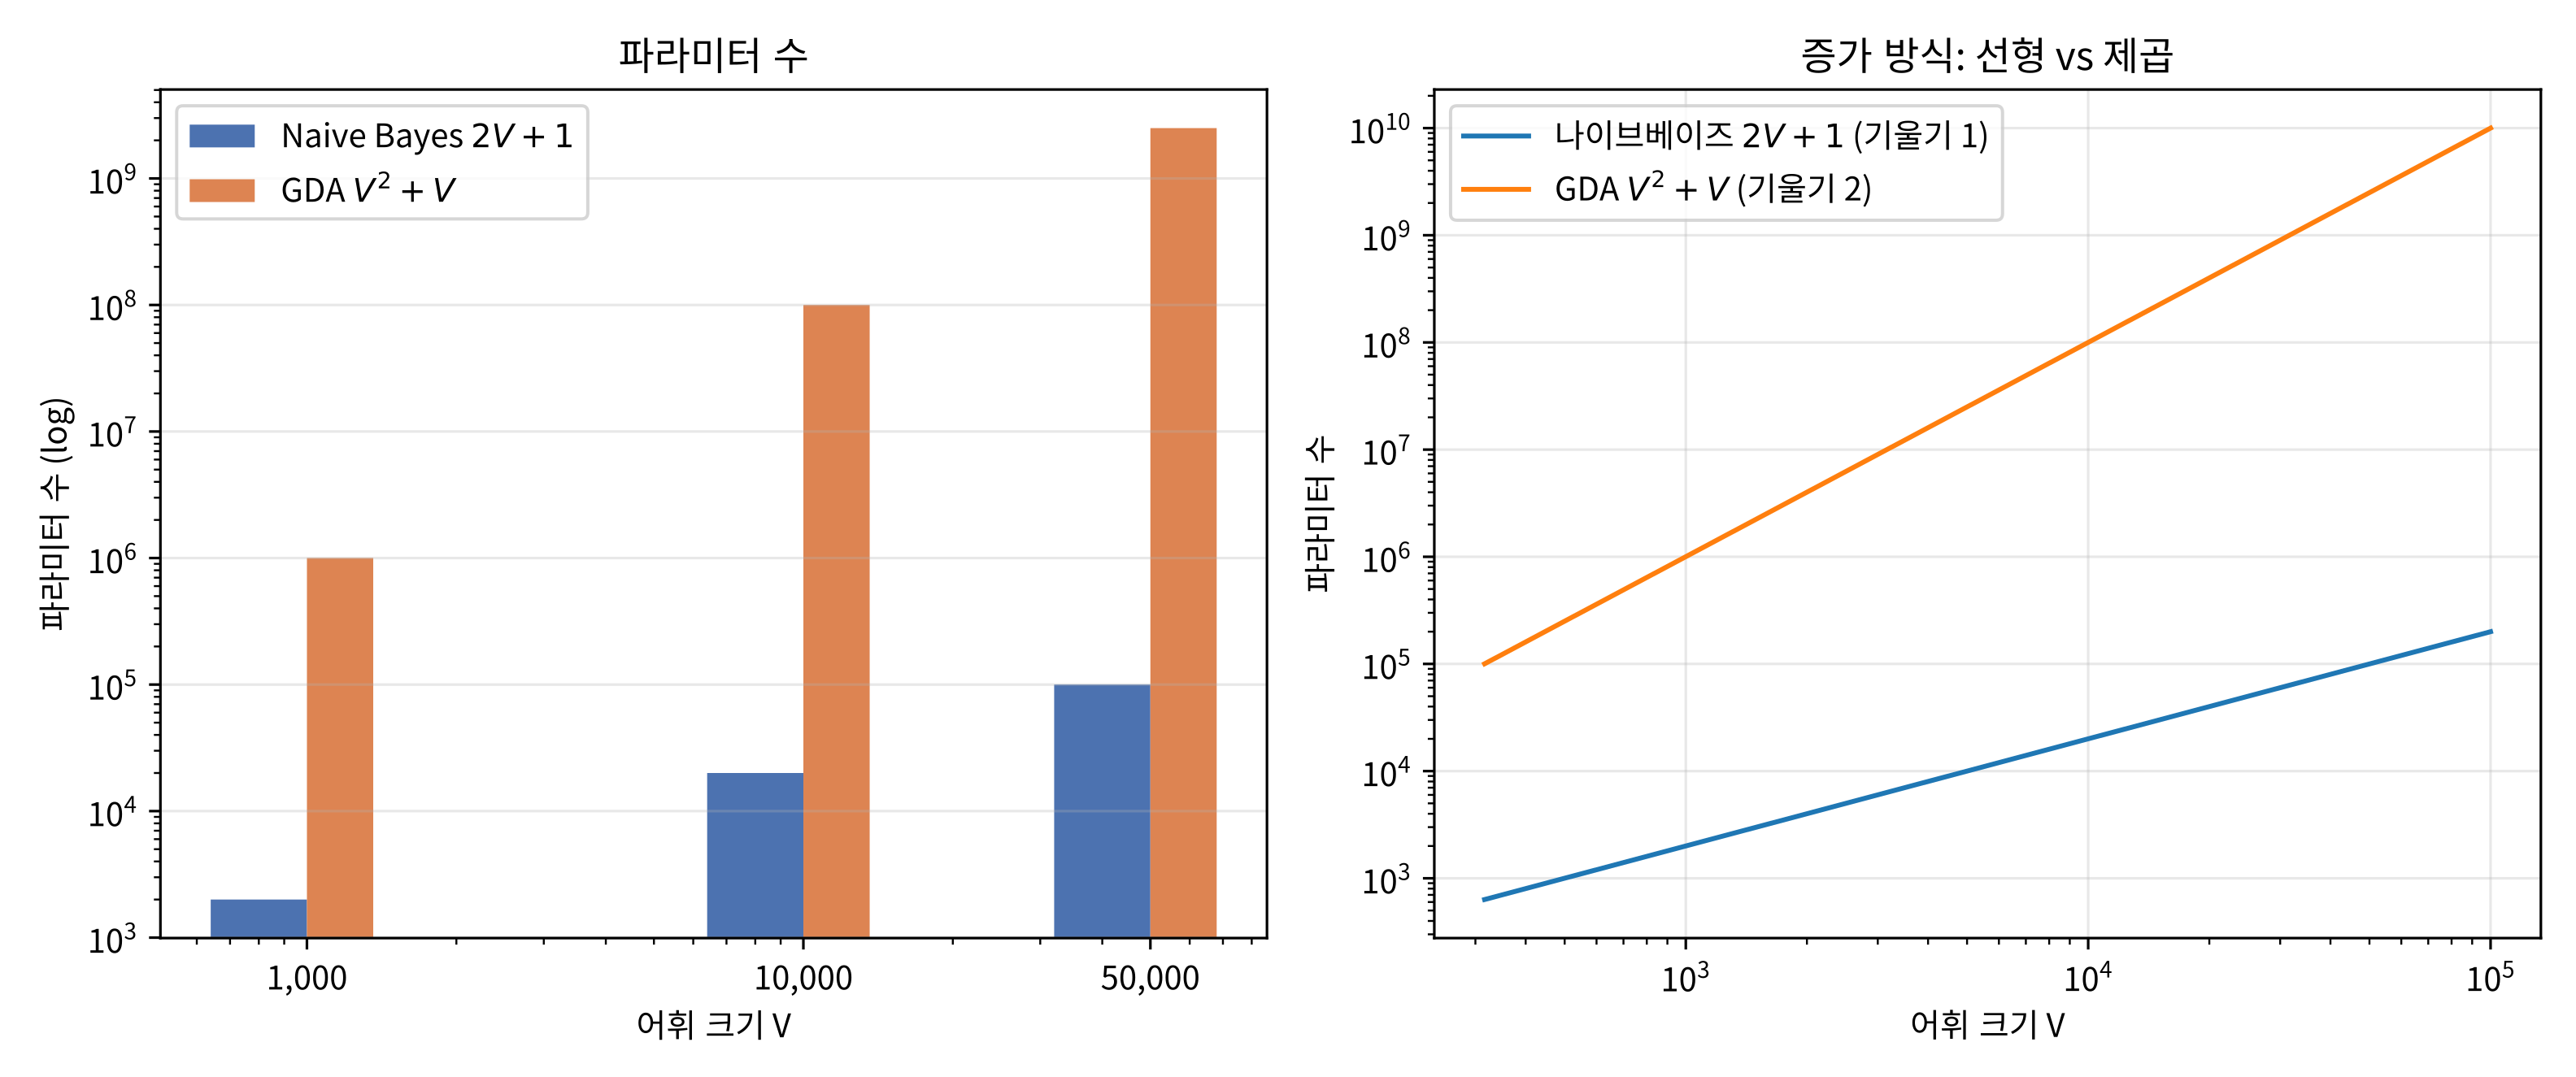
\includegraphics[width=0.85\linewidth]{ch03_naivebayes_paramcount.png}
      \\[0.2em]{\footnotesize 선형 vs 제곱.}
    \end{column}
  \end{columns}
\end{frame}

\begin{frame}{왜 ``증가 방식''이 품질을 좌우하나}
  \begin{itemize}
    \item 파라미터는 데이터에서 \textbf{계산해서} 얻는 값 ---
      표본에 비해 파라미터가 많으면 추정치가 실제 값 근처가 아니라
      \textbf{노이즈 근처}를 둥굴림.
    \item $\Sigma$ 의 각 원소 = ``단어 $i$ 와 단어 $j$ 가 얼마나
      \textbf{함께} 변하는가''의 추정치 --- 메일 수천 통으로
      \textbf{수백만 개}를 세면 전부 ``노이즈에 대한 추정''이 됨.
    \item \kb{차원의 저주}(Ch.\,4)가 분류기에 물리치는 전형적 방식.
    \item 나이브베이즈는 $\Sigma$ 의 \textbf{모든 옳각성분을 0로
      선언}(= 독립 가정)으로 원천 회피.
    \item \textbf{정확히는 틀린 가정}이지만, ``틀려도 안전한 방향''
      --- 상관 전부를 무시하고 \textbf{대각선만 정확히 세는} 쪽이
      차원이 크면 거의 항상 이득.
  \end{itemize}
\end{frame}

\begin{frame}{의존성을 무시해도 되는 이유: 과대평가의 방향}
  \begin{itemize}
    \item `무료'와 `당첨'은 실제로 \textbf{독립 아님}(스팸에서 함께
      나올 확률 높음).
    \item 나이브베이즈는 가능도를
      $P(\text{무료}|\text{spam})\times P(\text{당첨}|\text{spam})$
      로 곱해 --- 실제로는 그보다 \textbf{더 큰 값}이 될 가능성을
      무시한 채 계산.
    \item 즉, 독립 가정은 ``같은 클래스 안의 증거가 쌓이면 쌓을수록''
      가능도를 \kb{과대평가}하는 \textbf{편향}(bias).
    \item \textbf{중요}: 이 과대평가가 \textbf{두 클래스 모두에
      동시에} 일어남 --- 정상 쪽의 상관(`회의'×`보고서')도 같은
      방식으로 과대평가.
    \item 두 클래스의 점수가 \textbf{비슷한 방향으로} 왜곡되면
      \textbf{순위}는 거의 안 바뀌고 --- ``둘 다 10\%씩 부풀렸을 때
      누가 이기나''는 원래 순서와 대개 동일.
  \end{itemize}
\end{frame}

\begin{frame}{안전장치가 항상 작동하지는 않는다}
  \kq{의존성의 방향이 두 클래스에서 \textbf{다르면} 순위가 뒤집힐 수
  있다.}
  \vskip0.5em
  \begin{itemize}
    \item 예: `무료'×`당첨'이 스팸에서 \textbf{강하게 함께} 나오지만,
      정상 메일에서는 `무료'가 나오면 `당첨'이 \textbf{안 나오는}
      (음의 상관) 패턴이면, 과대평가 크기가 클래스마다 달라져
      \textbf{스팸 점수만 불리하게} 부풀어 오름.
    \item 실전에선 이런 패턴은 \textbf{드묾} (스팸/정상 모두
      ``비슷한 단어가 뭉쳐 나오는'' 구조를 공유하는 경우가 많음).
    \item 정확한 이해: ``나이브베이즈가 \textbf{영원히} 틀리지
      않는다''가 아니라, \textbf{틀리더라도 대개 \textbf{동일한
      방향}으로 틀린다}.
  \end{itemize}
\end{frame}

\begin{frame}{간단한 역사: 스펠링 수정기에서 스팸 필터까지}
  나이브베이즈가 실용화된 역사는 스팸보다 \textbf{한 세대 앞}:
  \begin{itemize}
    \item 1980년대 후반$\sim$1990년대: \kb{Peter Norvig}와
      Peter Fellbaum 등 --- \kb{자동 스펠링 수정}.
    \item 모델: $P(\text{타자 오류}|\text{정답 단어})
      \cdot P(\text{정답 단어})$ --- ``타자 오류'' = 인접 키/유사
      철자, ``정답 단어'' = 사전 빈도로 \textbf{독립} 가정.
      (2.3절 Viterbi의 전신이기도 함.)
    \item 2002년: \kb{Paul Graham} ``A Plan for Spam''으로 대중화 ---
      (1) 스팸 사전확률이 시간 경과로 변해 \textbf{클래스 비율로
        계속 갱신}, (2) 단어 하나만으론 부족 --- \textbf{모든 단어의
        로그 가능도를 더할 것}.
    \item 이 두 가지는 3.1 ``기저율 오류를 피하라''와 3.3 ``로그를
      더하라''와 \textbf{정확히 겹침}.
    \item ``독립 가정 + 빈도 카운팅''은 스펠링 $\to$ 스팸 $\to$
      텍스트 분류(감성·주제) $\to$ 의문문 감지 $\to$ 챗봇 의도
      분류까지 \textbf{기본 baseline} --- ``우선 나이브베이즈를
      돌려보라''가 실전 습관의 출발점.
  \end{itemize}
\end{frame}

\begin{frame}{다항 vs 베르누이: 독립 가정의 두 버전}
  \begin{columns}[T]
    \begin{column}{0.5\textwidth}
      \kb{베르누이 나이브베이즈}
      \begin{itemize}
        \item $x_j \in \{0,1\}$ --- ``단어 $j$ 가 \textbf{등장했는가}''
        \item 문서 \textbf{길이와 무관} (`free' 1번이든 10번이든
          ``등장 1건'')
        \item 길이가 신호인 문제(짧은 제목 vs 긴 본문)에 유용.
      \end{itemize}
    \end{column}
    \begin{column}{0.5\textwidth}
      \kb{다항(Multinomial) 나이브베이즈}
      \begin{itemize}
        \item $x_j$ = ``단어 $j$ 가 \textbf{몇 번} 나왔는가''
        \item $P(x|y) = \prod_j P(x_j|y)^{x_j}$ (다항분포)
        \item `free' 10번 메일 $>$ 1번 메일처럼 보고 싶을 때
          (대부분의 스팸/감성 분석) \textbf{자연스러움}.
      \end{itemize}
    \end{column}
  \end{columns}
  \vskip0.6em
  \begin{block}{공통}
    둘 다 ``클래스가 주어지면 단어들이 독립'' + \textbf{빈도 추정}의
    같은 구조. 실전에선 보통 다항이 더 잘 됨
    (scikit-learn \texttt{MultinomialNB}). 이번 절 코드는
    \textbf{베르누이} (교육적으로 단순).
  \end{block}
\end{frame}

\begin{frame}[fragile]{실습: 나이브베이즈 스팸 필터 (베르누이)}
  \begin{lstlisting}
import math

def train_naive_bayes(emails, labels):
    # emails: 단어 리스트의 리스트, labels: 0(정상)/1(스팸)
    vocab = set(w for email in emails for w in email)
    n_spam = sum(1 for l in labels if l == 1)
    n_ham = len(labels) - n_spam
    word_counts = {0: {}, 1: {}}
    for email, label in zip(emails, labels):
        for w in set(email):  # 등장 여부만 세는 Bernoulli 나이브베이즈
            word_counts[label][w] = word_counts[label].get(w, 0) + 1
    return {"vocab": vocab, "word_counts": word_counts,
            "n_spam": n_spam, "n_ham": n_ham, "n_total": len(labels)}

def classify(email, model):
    words = set(email)
    log_prob = {}
    for label, n_docs in [(0, model["n_ham"]), (1, model["n_spam"])]:
        log_p = math.log(n_docs / model["n_total"])   # log P(y)
        for w in model["vocab"]:
            p_present = (model["word_counts"][label].get(w, 0) + 1) / (n_docs + 2)
            log_p += math.log(p_present) if w in words else math.log(1 - p_present)
        log_prob[label] = log_p
    return 1 if log_prob[1] > log_prob[0] else 0
  \end{lstlisting}
  {\footnotesize 라플라스 스무딩 $(+1)/(+2)$ 적용, 모든 단어의
  $\log P(x_j|y)$ 를 \textbf{더함}.}
\end{frame}

\begin{frame}[fragile]{다항 버전: 8+8 학습, 4통 테스트}
  \begin{lstlisting}
import math

def train_multinomial_nb(emails, labels):
    vocab = sorted(set(w for e in emails for w in e))
    counts, nwords, ndocs = {0: {}, 1: {}}, {0: 0, 1: 0}, {0: 0, 1: 0}
    for e, l in zip(emails, labels):
        ndocs[l] += 1
        for w in e:                       # 이번엔 등장 횟수까지 센다
            counts[l][w] = counts[l].get(w, 0) + 1
            nwords[l] += 1
    return {"vocab": vocab, "counts": counts,
            "nwords": nwords, "ndocs": ndocs, "n_total": len(labels)}

def multinomial_log_probs(email, model):
    out = {}
    for l in (0, 1):
        lp = math.log(model["ndocs"][l] / model["n_total"])
        for w in email:
            p = (model["counts"][l].get(w, 0) + 1) / \
                (model["nwords"][l] + len(model["vocab"]))   # 라플라스
            lp += math.log(p)
        out[l] = lp
    return out
  \end{lstlisting}
\end{frame}

\begin{frame}[fragile]{4/4 모두 올바르게}
  \begin{lstlisting}
spam_train = ["free money now", "win prize today", "free cash click",
              "prize free offer", "money win now", "free click here",
              "prize cash deal", "offer win cheap"]
ham_train = ["meeting project tomorrow", "project deadline review",
             "team meeting report", "meeting notes call", "project update plan",
             "report review friday", "team lunch call", "meeting agenda notes"]

emails = spam_train + ham_train
labels = [1]*8 + [0]*8
model = train_multinomial_nb(emails, labels)

test_emails = [
    ("free prize money", 1),        # 학습에서 보지 못한 스팸 조합
    ("win click offer", 1),
    ("meeting project report", 0),  # 학습에서 보지 못한 정상 조합
    ("team call notes", 0),
]
for email, truth in test_emails:
    lp = multinomial_log_probs(email.split(), model)
    pred = 1 if lp[1] > lp[0] else 0
    print(f"{'SPAM' if truth else 'HAM ':4s} pred={pred} "
          f"margin={abs(lp[1]-lp[0]):.2f} nats  {email!r}")
  \end{lstlisting}
  \vskip0.1em
  {\footnotesize 4/4 정답: \texttt{SPAM pred=1 margin=4.09 / 3.58},
  \texttt{HAM pred=0 margin=4.09 / 3.30} (nat).}
\end{frame}

\begin{frame}{margin: ``자신 있는 예측''의 수치}
  \begin{itemize}
    \item \kb{margin} = 로그 점수 차이, nat 단위 --- 실전적으로
      \textbf{중요한 지표}.
    \item margin 4.09 nat = $e^{4.09}\approx 60$ 배 가능도비 ---
      ``거의 확실하게 스팸''.
    \item margin 0.3 nat = $e^{0.3}\approx 1.35$ 배 --- ``거의
      동점'' $\Rightarrow$ 데이터가 약간만 바뀌어도 뒤집힐 수 있음.
    \item \textbf{정확도(맞은 비율)뿐 아니라 margin 분포까지 봄}이
      예측을 신뢰하는 방식.
    \item margin이 \textbf{작은 메일만} 골라 ``모델이 가장 자신
      없어하는 예시''를 분석하면, 데이터셋에 어떤 패턴이 부족한지(또는
      레이블 오류가 있는지) 빠르게 드러남.
  \end{itemize}
\end{frame}

\begin{frame}{손으로 한 번: 2-단어 어휘 NB}
  어휘 = \{`공짜', `회의'\}. 학습: 스팸 \{\{공짜\},
  \{공짜, 회의\}\}, 정상 \{\{회의\}, \{회의\}\}.
  새 메일 \{\textbf{공짜}\} (``공짜''만 있고 ``회의''는 없음):
  \vskip0.4em
  $P(y)$ 는 양쪽 $2/4=0.5$. \kb{라플라스 스무딩}을 적용한 가능도:
  \[ P(\text{공짜 있음}|\text{spam}) = \frac{2+1}{2+2} = 0.75, \hspace{2em}
     P(\text{회의 없음}|\text{spam}) = 1 - \frac{1+1}{2+2} = 0.5 \]
  \[ P(\text{공짜 있음}|\text{ham}) = \frac{0+1}{2+2} = 0.25, \hspace{2em}
     P(\text{회의 없음}|\text{ham}) = 1 - \frac{2+1}{2+2} = 0.25 \]
  \vskip0.3em
  정규화 전: 스팸 $0.5\times0.75\times0.5 = \textbf{0.1875}$ vs
  정상 $0.5\times0.25\times0.25 = 0.03125$.
\end{frame}

\begin{frame}{$\{\text{공짜}\}$ 의 사후확률 = 0.857}
  \[ P(\text{spam}|\{\text{공짜}\})
     = \frac{0.1875}{0.1875+0.03125} \approx \textbf{0.857} \]
  \vskip0.4em
  \begin{block}{한 단어로 85.7\%}
    `공짜' \textbf{단 하나}로 스팸 확률이 85.7\%까지 도약
    (가능도비 6:1). 3.1절의 베이즈 계산과 \textbf{완전히 같은 절차},
    다만 곱해지는 증거가 `공짜 있음' + `회의 없음' 두 개로 늘어난 것 ---
    실제 필터는 어휘 전체(수만 개)에 대해 이 곱을 전부 수행.
  \end{block}
\end{frame}

\begin{frame}{네 가지 메일: 경계의 지도}
  같은 학습 데이터로 4개 메일을 분류:
  \small
  \begin{tabular}{@{}lcll@{}}
    \toprule
    메일 & $P(\text{spam}|x)$ & 예측 & 직관 \\
    \midrule
    $\{$공짜$\}$ & \textbf{0.857} & 스팸 & `공짜': 스팸 2/2, 정상 0/2 \\
    $\{$공짜, 회의$\}$ & 0.667 & 스팸 & `공짜'가 스팸 쪽으로 끌고, `회의'(양쪽 1/2)가 약한 정상 신호 \\
    $\{$회의$\}$ & 0.182 & 정상 & `회의'만 있으면 정상($0.5\times0.25\times0.75=0.09375$)이 스팸($0.5\times0.5\times0.25=0.0625$)을 이김 \\
    $\varnothing$ (없음) & 0.400 & 정상 & 사전확률(0.5)과 `단어 없음' 신호(약한 스팸)가 부분 상쇄 \\
    \bottomrule
  \end{tabular}
  \vskip0.6em
  {\footnotesize 2행이 흥미로움: `회의'는 양쪽 모두에 나타나되
  \textbf{정상에 더 자주}(2/2 vs 1/2) $\Rightarrow$ 약한 \textbf{정상
  신호}. `공짜'의 강한 스팸 신호(0.75 vs 0.25, 3배)와 `회의 없음'의
  약한 스팸 신호(0.5 vs 0.25, 2배)가 합쳐져 스팸 $0.5\times0.75\times
  0.25 = 0.09375$ > 정상 $0.5\times0.25\times0.5 = 0.0625$.
  개별 단어가 ``스팸/정상 단어''로 딱 떨어지지 않아도,
  \textbf{로그를 더하며 신호가 적립} --- ``단어 하나가 아니라 전체
  메일을 본다''는 NB의 본질.}
\end{frame}

\begin{frame}{자주 하는 실수: 카운트 방식 선택}
  코드의 \texttt{for w in set(email)} 는 같은 단어가 여러 번 나와도
  \textbf{한 번만} 센다(베르누이) --- 실전에선 이 선택 자체가 버그의
  원인:
  \begin{itemize}
    \item `free' 10번 메일은 분명 1번 메일보다 스팸 가능성이 높은데,
      \texttt{set(email)} 은 \textbf{동일하게 처리} --- 신호 9개를
      버림.
    \item 반대로, \textbf{단어 수로 정규화하지 않은 채} 횟수만 곱해
      버리면(다항 + 스무딩 없음), \textbf{긴 메일일수록} 모든
      확률 곱이 무조건 작아져서 \textbf{문서 길이가 예측에 영향}
      을 주는 엉뚱한 인과가 생김.
    \item ``등장 \textbf{여부만} 볼 것인가(베르누이), \textbf{횟수}
      까지 볼 것인가(다항), 볼 때 어떻게 정규화할 것인가''를
      \textbf{의식적으로} 정하고, 데이터셋 특성(길이가 신호인가,
      반복 빈도가 신호인가)에 맞게 고를 것.
  \end{itemize}
\end{frame}

\begin{frame}{자주 하는 실수: 스무딩 없이 곱하기}
  \kq{학습에서 못 본 단어 하나면 \textbf{전체 곱이 0}으로 강제됨.}
  \vskip0.4em
  \begin{itemize}
    \item 예: `당첨'이 정상 메일에 \textbf{한 번도} 없으면
      $P(\text{당첨}|\text{ham}) = 0/n_{\text{ham}} = \textbf{0}$.
    \item 새 메일에 `당첨'이 등장하는 순간, 그 메일이 다른 단어들로 볼
      때 아무리 정상 메일에 가까워 보여도
      $P(\text{ham})\times\cdots\times\textbf{0}\times\cdots = 0$
      --- \textbf{단어 하나가 다른 모든 증거를 무시하고 결론을
      독단}.
    \item \kb{라플라스 스무딩}($+1 / +2$) = ``못 본 조합이라고
      확률이 \textbf{정확히 0}이라 단정하지 않는다''는 보수적
      가정을 수학적으로 표현.
    \item \textbf{데이터가 적을수록} 스무딩 영향이 큼
      ($n{=}2,3$이면 $+1$이 결과를 크게 바꿈), 크면 무시할 수준.
  \end{itemize}
\end{frame}

\begin{frame}{스무딩 효과 숫자로: `당첨'이 들어온 메일}
  앞의 학습 데이터(어휘 \{공짜, 회의\})에서 \textbf{한 번도 보지
  못한} `당첨'이 포함된 새 메일 $\{$공짜, \textbf{당첨}$\}$:
  \vskip0.3em
  \small
  \begin{tabular}{@{}lll@{}}
    \toprule
     & $P(\text{당첨 있음}|\text{spam})$ & $P(\text{당첨 있음}|\text{ham})$ \\
    \midrule
    \textbf{스무딩 없이} & $0/2 = \textbf{0}$ & $0/2 = \textbf{0}$ \; $\Rightarrow$ 0 vs 0 \textbf{비교 불가} \\
    \textbf{라플라스} & $1/4$ & $1/4$ \; $\Rightarrow$ \textbf{중립} 신호 \\
    \bottomrule
  \end{tabular}
  \vskip0.8em
  \begin{itemize}
    \item 스무딩을 쓰면 `당첨'은 \textbf{중립}이 되고, 남은 `공짜'
      (스팸 3/4 vs 정상 1/4)이 판단을 결정:
      $P(x|\text{spam}) = \tfrac34\times\tfrac14 = 0.1875$,
      $P(x|\text{ham}) = \tfrac14\times\tfrac14 = 0.0625$
      --- `공짜'가 본래 가질 \textbf{3배의 증거}(0.1875/0.0625)를
      그대로 살려 \textbf{스팸}으로 분류.
    \item ``0/0 비교 불가''에서 ``3:1로 스팸''으로 바뀌는 것 ---
      스무딩은 ``확률 0의 사건''을 ``아직 관찰되지 않았을 뿐, 매우
      희소할 것''으로 \textbf{재정의}.
  \end{itemize}
\end{frame}

\begin{frame}{사전확률 $P(y)$ 의 힘: 그레이엄의 ``스팸이 90\%''}
  NB 점수 $\log P(y) + \sum_j \log P(x_j|y)$ 의 \textbf{첫 항}
  $\log P(y)$ 가 바로 사전확률 --- 기저율 오류가 그대로 적용.
  \vskip0.4em
  앞의 학습 데이터로 만든 NB에서, \textbf{가능도가 전혀 도움이 안
  되는} 메일 $\{$공짜, 회의$\}$ 를 분류:
  \[ P(\text{공짜}|\text{spam})\,P(\text{회의}|\text{spam})
     = \tfrac34\times\tfrac12 = \tfrac38 = \tfrac14\times\tfrac34
     = P(\text{공짜}|\text{ham})\,P(\text{회의}|\text{ham}) \]
  \vskip0.2em
  가능도비는 정확히 \textbf{2}(스팸 쪽) --- ``스팸도 정상도 똑같이
  잘 설명'' $\Rightarrow$ 분류는 \textbf{완전히 $P(y)$ 로 결정}.
\end{frame}

\begin{frame}{가능도비 2: 사전확률이 예측을 뒤집음}
  \small
  \begin{tabular}{@{}lcl@{}}
    \toprule
    학습된 스팸 비율(사전확률) & $P(\text{spam}\mid\{$공짜, 회의$\})$ & 예측 \\
    \midrule
    50\% & 0.667 & 스팸 (\textbf{불확실하게}) \\
    90\% & 0.947 & 스팸 (\textbf{거의 확실하게}) \\
    10\% & \textbf{0.182} & \textbf{정상} (예측 뒤집힘) \\
    \bottomrule
  \end{tabular}
  \vskip0.8em
  \begin{itemize}
    \item 가능도비 2처럼 \textbf{동점 쪽}에 쏠린 메일에서는
      ``스팸이 흔한 시대에 살고 있는가''가 판단을 좌우.
    \item 90\%에선 0.947로 거의 확실, 10\%에선 0.182로
      \textbf{완전히 뒤집힘} --- 단어 증거의 2:1 우위가
      사전확률의 \textbf{9:1}에 밀림.
    \item 2002년 스팸 현실(메일함 스팸 비율 수십 \%)에 정확히
      맞닿음 --- 그레이엄은 ``적응적 필터'': $P(y)$ 를
      \textbf{클래스 비율로 계속 갱신}.
    \item 반대로 스팸이 드문 환경(내부 사내 메일)이면 같은 `공짜'
     라도 덜 민감하게 반응해야 --- $P(y)$ 를 \textbf{학습 데이터의
      클래스 비율}로 정확히 넣어야 균형이 자동 조정.
  \end{itemize}
\end{frame}

\begin{frame}{확인 문제: 사전확률만으로 뒤집히는 메일}
  \begin{itemize}
    \item \textbf{(a)} 같은 학습 데이터에서, 사전확률
      \textbf{50/50}과 \textbf{90/10}(스팸/정상)일 때의
      $P(\text{spam}\mid\{$회의$\})$ 를 라플라스 스무딩으로 계산 ---
      어느 쪽에서 `회의'만 있는 메일을 \textbf{스팸}으로 분류하게 되는가?
      그 차이가 사전확률 $\log\frac{0.9}{0.1}\approx2.2$ nat에서
      오는 것인지, 가능도에서 오는 것인지 \textbf{구별}.
      {\footnotesize 답: 50/50 $\to$ 0.40 (정상), 90/10 $\to$
      $\frac{0.9\times0.5}{0.9\times0.5+0.1\times0.75}\approx0.857$
      (스팸). 가능도비 2/3은 동일, 바뀐 건 \textbf{사전확률 우위
      9:1}.}
    \item \textbf{(b)} 가능도비 $r$ 로 쓸 때: 50/50에서 정상 예측
      $\Leftrightarrow r<1$, 90/10에서 스팸 예측 $\Leftrightarrow
      9r>1 \Leftrightarrow r>1/9$.
      \vskip0.2em
      \textbf{$1/9 < r < 1$}인 메일만 50/50 $\to$ 90/10 변화로
      뒤집힘. 예: $r{=}0.5$ 면 1/3(정상) $\to$ 0.818(스팸).
      반대로, $r{=}2$(스팸 쪽)인 메일은 50/50 $\to$ 10/90 방향에서만
      뒤집힘. 한 문장: \textbf{가능도비가 1 근처($\sim$1/9 $\sim$ 9)인
      ``동점이 가까운'' 메일만, 사전확률의 9:1 변화에 의해 뒤집힘}.
  \end{itemize}
\end{frame}

\begin{frame}{왜 로그를 더하는가: 언더플로우 방지}
  \begin{itemize}
    \item 단어가 수천 개면 $P(x_j|y)$ 를 수천 번 곱하면
      \textbf{극도로 작은 수} $\to$ 부동소수점 정밀도로 구분 불가
      (\kb{underflow}).
    \item Ch.\,2 교차 엔트로피가 확률 곱 대신 로그 합을 쓴 것과
      \textbf{정확히 같은 이유}:
      \[ \log\prod_j P(x_j|y) = \sum_j \log P(x_j|y) \]
    \item \textbf{숫자로}: float64는 $\approx10^{-308}$ 이하가
      \textbf{정확히 0.0}으로 떨어짐.
      어휘 $V{=}2000$에서 단어당 0.98이면
      $0.98^{2000}\approx2.8\times10^{-18}$ --- 아직 살아있음.
      $V{=}200{,}000$이면 $0.98^{200000}=\textbf{0.0}$ ---
      \textbf{양 클래스 가능도 모두 0.0}, 비교 불가.
    \item \textbf{로그 공간}에서는 $200{,}000\times\log 0.98
      \approx -4041$로 \textbf{유한}, 스팸 $-4041$ vs 정상 $-4364$
      같은 비교가 평범하게 동작.
    \item ``정확한 확률값''($\approx10^{-1755}$)은 분류에 쓰이지도
      않는 \textbf{의미 없는 값} --- \textbf{두 로그 점수의 차이}만
      의미. 실제 구현은 확률 곱을 \textbf{한 번도 만들지 않고}
      처음부터 로그만 쌓음.
  \end{itemize}
\end{frame}

\begin{frame}{자주 묻는 질문 (3.3)}
  \begin{itemize}
    \item \textbf{Q. 독립 가정이 명백히 틀렸는데 왜 잘 되나?}
      분류는 \textbf{정확한 확률값}을 완벽히 맞힐 필요가 없고
      \textbf{어느 클래스 점수가 큰가}(순위)만 맞히면 됨.
      의존성 무시로 확률값이 왜곡돼도, 그 왜곡이 \textbf{두 클래스
      모두에 비슷한 방향}으로 일어나는 경우가 많아서
      \textbf{상대 순위}가 크게 안 틀림.
    \item \textbf{Q. 텍스트 데이터엔 뭘 써야 하나?} \textbf{거의
      항상 나이브베이즈} --- 어휘가 수만이면 GDA의 $\Sigma$
      (어휘 크기 \textbf{제곱} 원소) 추정에 데이터가 절대 부족.
      반대로 \textbf{저차원 연속값}(키·몸무게 등)이면 GDA가
      특징 간 상관(공분산)까지 반영해 유리.
    \item 실전 고르는 기준: \textbf{``특징이 많고 이산적? $\to$
      NB. 적고 연속? $\to$ GDA.''}
      더 깊이: Stanford CS229 노트.
  \end{itemize}
  \vskip0.6em
  \begin{block}{3.2 + 3.3의 공통 철학}
    GDA(연속값에 정규분포)와 NB(이산값에 독립 가정)는 접근 방식은
    달라도, \textbf{둘 다 ``먼저 각 클래스가 데이터를 어떻게
    만드나를 모델링하고, 베이즈 정리로 뒤집는다''는 생성적 철학}을
    공유.
  \end{block}
\end{frame}

% ===== wrap-up =====
\begin{frame}{이번 주차 정리}
  \small
  \begin{enumerate}
    \item \kb{3.1 베이즈 정리 = ``같은 $P(x,y)$ 를 앞뒤로 나누는''}
      \hbox{}\\
      세 단어(사전·가능도·사후) + ``세로 합 = 조건부 세계'' 확률
      트리. \textbf{오즈 = 가능도비 곱의 연쇄}가 NB의 로그 합과
      로지스틱 시그모이드를 같은 자리에서 설명. \textbf{기저율
      오류}: 사전확률을 빼먹으면 99\% 검진도 9\% 사후확률.
    \item \kb{3.2 GDA = 가우시안 + 공유 공분산 + MLE}
      \hbox{}\\
      평균·공분산으로 \textbf{닫힌 형태}. 이차항 상쇄 $\Rightarrow$
      \textbf{결정 경계는 항상 직선}. $P(y{=}1|x)=\sigma(w^\top x+b)$
      --- \textbf{로지스틱회귀와 같은 시그모이드}. $\phi$ 는
      위치만 미는 \textbf{병렬 이동} = 경계의 기저율 오류.
    \item \kb{3.3 NB = 독립 가정 + 빈도 카운팅}
      \hbox{}\\
      파라미터 \textbf{선형}($2V{+}1$) vs GDA \textbf{제곱}($V^2{+}V$)
      $\Rightarrow$ \textbf{차원의 저주 회피}. 틀려도 \textbf{동일한
      방향}으로 틀려 순위 유지. 스무딩(0 강제 방지) · \textbf{로그
      합}(언더플로우) · \textbf{사전확률}(가능도비 2도 10\%면 뒤집힘).
  \end{enumerate}
  \vskip0.8em
  \begin{block}{다음 주 --- Chapter 4. kNN과 k-means}
    또 다른 극단: \textbf{배울 파라미터가 전부 없는} 분류기.
    ``$k$개 가장 가까운 이웃을 보고 다수결'' --- ``모델 없이
    거리만으로''. 이번 장의 ``데이터 생성 법칙을 배운다''에서
    ``아무것도 배우지 않는다''로 넘어가는 것. 다만 이번 장이 예고한
    \textbf{차원의 저주}는 Ch.\,4에서 ``왜 kNN이 고차원에서 무너지는가''
    로 다시 나옴.
  \end{block}
\end{frame}

\end{document}
